\documentclass{beamer}
\usetheme{afm}

\title{Interest Rate Derivatives}
\subtitle{Main Ineterst Rate Contracts Theory}
\course{Advanced Financial Modelling}
\author{\href{mailto:matteo.sani@unisi.it}{Matteo Sani}}

\begin{document}
\begin{frame}[plain]
  \maketitle
\end{frame}

\begin{frame}{Single Curve Approach}
	\begin{block}{Disclaimer}
	What follows is a detailed exposition of the classic \textcolor{red}{single curve}
	approach for interest rate derivatives. 
	
	Today a \textcolor{red}{multi-curve approach} is
	used in practical applications. Nevertheless you need to understand
	deeply this basic approach as a prerequisite for the extension to the
	multi-curve model.
	\end{block}
\end{frame}  

\subsection{Money Market Account}
\begin{frame}{Money Market Account}
	\begin{itemize}
		\item<0-> The \textcolor{red}{money market account} represents a risk-less investment, where profit is accrued continuously at the risk-free rate, and its value is denoted by $B(t)$.
		\item<1-> We assume $B(0)=1$ and by definition
		\begin{equation}
			dB(t) = r(t)B(t)dt
		\end{equation}
		\item<2-> This evolution can be solved through variable separation
		\begin{equation}
			\begin{gathered}
				\frac{dB_t}{B_t} = r_t dt \implies \int_0^t \frac{dB_t}{B_t} = \int_0^t r_s ds \\
				\implies \log\frac{B_t}{B_0} = \int_0^t r_s ds \implies \boxed{B(t) = \exp\left(\int_0^t r_s ds\right)}
			\end{gathered}
		\end{equation}
		where $r_t$ is referred to as \textcolor{red}{instantaneous spot rate} or \textcolor{red}{short rate}.
	\end{itemize}
\end{frame}

\begin{frame}{Money Market Account}
	\begin{itemize}
		\item<0-> The \emph{short rate} $r_t$ can be modeled either by a deterministic or a stochastic process.
		\item<1-> \textbf{Deterministic case}: from the definition of money market account, if I have $A$ units of currency at time 0, it follows that 
		\begin{equation*}
			V(0) = A\cdot B(0) \implies V(t) = A\cdot B(t)
		\end{equation*}
		\item<2-> If we want to have at time $T$ exactly 1 unit of currency
		\begin{equation*}
			AB(T) = 1 \implies A = \frac{1}{B(T)} \implies AB(t) = \frac{B(t)}{B(T)} 
		\end{equation*}
		hence $\frac{B(t)}{B(T)}$ is \textcolor{red}{the value of one unit of currency payable at time $T$ seen from $t$}.
		
		%%		\item We now define the abstract quantity $r(t)$, the \textbf{short rate}, as
		%%		\begin{equation}
			%%			r(t) = \lim_{T\rightarrow t^+} L(t,T) \simeq L(t, t+\epsilon)
			%%		\end{equation}\quad with $\epsilon$ small
	\end{itemize}
\end{frame}

\subsection{Stochastic Discount Factor and Zero Coupon Bond}
\begin{frame}{Stochastic Discount Factor}
	\uncover<1->{
		\begin{block}{Definition}
			The \textcolor{red}{(stochastic) discount factor} $D(t, T)$ is the amount at time $t$ that is \emph{equivalent} to one unit of currency payable at time $T$ and is given by
			\begin{equation}
				D(t, T) = \frac{B(t)}{B(T)} = e^{-\int_t^T r_s ds}
			\end{equation}
	\end{block}}
	\begin{itemize}
		\item<2-> Can you guess what is the unit of measurement of a discount factor ?	
		\item<3-> In many pricing application (e.g. Black-Scholes formula) $r$ is assumed to be a \textcolor{red}{deterministic} function of time, and so are $B(t)$ and $D(t,T)$:
		\begin{itemize}
			\item<3-> this is motivated by the small influence interest rate variations have on equity prices.
		\end{itemize}
		\item<4-> When dealing with interest rate products, $r$ becomes the main actor, so the deterministic assumption must be dropped.
	\end{itemize}	
\end{frame}

\begin{frame}{Deterministic vs Stochastic}
	\begin{itemize}
		\item<0-> Recall the risk-neutral pricing formula \begin{equation*}
			\Pi_t = \expect{Q^B}[D(t,T)A|\mathcal{F}_t]
		\end{equation*}
		where the corresponding risk-neutral measure is often denoted by $\mathbb{Q}^0$ or $\mathbb{Q}^B$, and similarly for the expectations. 
		%	In the following we are going to use $B(t)$ as numeraire then  Eq.~\ref{eq:risk_neutral_pricing} becomes
		%	\begin{equation*}
			%		\begin{aligned}
				%			S_t = \mathbb{E}^{\mathcal{Q}^B}\left[e^{-\int_t^T r_s ds}S_T|\mathcal{F}_t\right]
				%		\end{aligned}
			%	\end{equation*}
		%	where $\mathcal{Q}^B$ is the risk-neutral measure.% that makes $\frac{S_t}{B_t}$ a martingale. 	
		\item<1-> When \textcolor{red}{interest rates are deterministic}, the exponential can be brought out of the expectation
		\begin{equation*}
			\Pi_t = e^{-\int_t^T r_s ds} \expect{B}\left[A|\mathcal{F}_t\right]
		\end{equation*}
		\item<2-> If in addition \textcolor{red}{rates are constant} (e.g. Black-Scholes or Heston models)
		\begin{equation*}
			\Pi_t = e^{-r(T-t)}\expect{B}\left[A|\mathcal{F}_t\right]
		\end{equation*}
	\end{itemize}
\end{frame}

\begin{frame}{Zero Coupon Bond}
	\begin{itemize}
		\item<1-> \textcolor{red}{Zero Coupon Bond} (ZCB) is a contract that pays one unit of money at time $T$. Its price at time $t$ is denoted by $P(t,T)$, and by definition $P(T,T) = 1$.
		\item<1-> What is the relation between $P(t,T)$ and $D(t,T)$ ? \\
	\end{itemize}
		\uncover<2->{
			\renewcommand{\arraystretch}{1.2}
			{\tiny {\tiny }}{
				\begin{table}[bt]
					\begin{tabular}{|c|c|} \hline
						$D(t, T)$ & $P(t, T)$ \\ \hline
						equivalent amount of money & value of a contract \\ \hline
						\multicolumn{2}{|c|}{\textcolor{red}{deterministic rates}} \\ \hline
						\multicolumn{2}{|c|}{$D(t,T)$=$P(t,T)$} \\ \hline 
						\multicolumn{2}{|c|}{\textcolor{red}{stochastic rates}} \\ \hline
						random quantity at time $t$ &
						\renewcommand{\arraystretch}{1.0} 
						\begin{tabular}{@{}c@{}}
							it has a payoff at time $T$, must be known in $t$ \\
							from 
							$P(t, T) = \expect{Q}[D(t, T)|\mathcal{F}_t]$
						\end{tabular} \\ \hline
					\end{tabular}
				\end{table}
		}}
\end{frame}

%\begin{frame}{Year Fraction, Day-Count Convention}
%	\begin{itemize}
%		\item Time to maturity: $T-t$
%		\item Denote by $\tau(t, T)$ the chosen time measure between $t$ and $T$. In theory, you can think of $\tau(t, T)=T-t$. In practice there are many possible ways to compute that time difference.
%		\item Among the plethora of conventions, the followings are worth mentioning:
%		\begin{itemize}
%			\item Actual/365
%			\item Actual/360
%			\item 30/360
%		\end{itemize}
%		\item \textcolor{red}{Go and find their definitions: they are also embedded in Excel as financial functions.}
%	\end{itemize}
%	\begin{tikzpicture}[remember picture,overlay]
%		\node[xshift=5cm,yshift=-3.7cm] (image) at (current page.center) {
\includegraphics[width=20px]{python_logo}};
%		\node[align = center, yshift=1.45cm, below=of image] {\tiny{\href{shorturl.at/chzT2}{shorturl.at/chzT2}}};
%	\end{tikzpicture}
%\end{frame}

\subsection{Spot Interest Rate}
\begin{frame}{Spot Interest Rate}
	\begin{itemize}
		\item Simply-compounded \textcolor{red}{spot interest rate}
		\begin{equation}
			L(t,T)=\frac{(1-P(t,T))}{\tau(t,T)P(t,T)}		
		\end{equation}
		represents the interest rate applicable to a single payment at a future date, calculated using simple interest
		\item The \textcolor{red}{yield curve} at time $t$ is the graph of:
		\begin{equation*}
			T\rightarrowtail L(t, T)
		\end{equation*}
		\item In the market these are the so called EURIBOR rates and are typically compounded with the actual/360 convention. They are the main rates underlying interest rate derivatives.
	\end{itemize}
\end{frame}

\section{Forward Rate Agreement}
\begin{frame}{Forward Rate Agreement}
	\begin{itemize}	
		\item<1-> A \textcolor{red}{Forward Rate Agreement} (FRA) is a contract involving three time instants: %the current time $t$, the fixing time $T>t$, and the maturity time $S>T$.
		\begin{equation*}
			\underbrace{t}_{\text{current time}} \leq \underbrace{T}_{\text{fixing time}} \leq\underbrace{S}_{\text{maturity}}
		\end{equation*}
		\item<2-> The FRA payout consists of an exchange of interest rate flows calculated for the time period $\tau=S-T$. At the maturity $S$, a fixed payment based on a fixed rate $K$ is exchanged against a floating payment based on the spot rate $L(T, S)$ whose value is known only in $T$.
		\item<3-> Basically, this contract allows one to lock-in the interest rate between times $T$ and $S$ at a desired value $K$.
		 
		\noindent
		(\textbf{note:} interest rate flows are calculated using the simple compounding law).
	\end{itemize}
\end{frame}

\begin{frame}{FRA Example}
	\begin{itemize}
	\item A FRA is an agreement that enables to \emph{hedge} against unfavourable movements in interest rates by fixing a rate on a notional amount that is (usually) of the same size and term as the exposure that starts sometime in the future. 
	\vfill
	\begin{center}
		\includegraphics[width=0.9\linewidth]{images/FRA_diagram}
	\end{center}
	\end{itemize}
\end{frame}

\begin{frame}{FRA Time Table}
	\begin{itemize}
		\item Consider a $1\times 3$ FRA (1-month into 3-month): the 1 in the $1\times 3$ refers to 1 month' time when settlement (fixing) takes place, and the 3 to the expiry date of the FRA from deal date.
		%, i.e. the rate quoted for the FRA is a 1-month rate at the time of settlement
	\begin{center}
		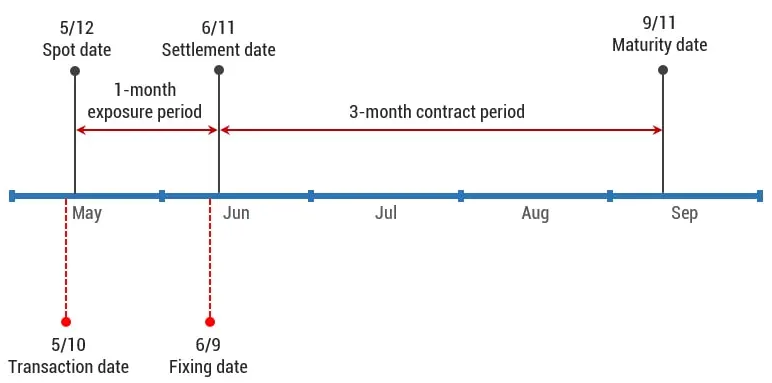
\includegraphics[width=0.8\linewidth]{images/fra_timeline}
	\end{center}
\end{itemize}
\end{frame}

\begin{frame}{FRA: Formalization of the Contract}
	\begin{itemize}
		\item<1-> Formally, at time $S$ one receives $\tau(T, S)KN$ units of currency and pays the amount $\tau(T,S)L(T,S)N$, where $N$ is the contract nominal value.
		\item<2-> Thus, at time $S$, the future (and \textbf{today unknown}) payout of the contract is: 
		\begin{equation}
			N\tau(T,S)(K-L(T,S))
			\label{eq:fra_payoff}
		\end{equation}
		\item<3-> In order to assign a \textbf{value} at this contract we have to tackle two issues:
		\begin{itemize}
			\item<3-> estimate the future value of $L(T, S)$;
			\item<3-> discount the result from $S$ to today (time $t$).
		\end{itemize}
		\item<4-> There are several ways to arrive at the final result: \textbf{no arbitrage is the common denominator.}
	\end{itemize}
\end{frame}

\subsection{FRA Valuation}
\begin{frame}{FRA: Brigo-Mercurio Approach}
	\begin{itemize}
		\only<1-1>{
		\item Substitute in \cref{eq:fra_payoff} $L(T,S)$ with its expression as a function of the zero-coupon bond price $P$ and get
		\begin{equation*}
			\mathbb{E}\left[D(t, S) N\bigg(\tau K + 1 - \frac{1}{P(T, S)}\bigg)\bigg| \mathcal{F}_t\right]
		\end{equation*}
		}
		\only<2->{
		\item Substitute in \cref{eq:fra_payoff} $L(T,S)$ with its expression as a function of the zero-coupon bond price $P$ and get
		\begin{equation*}
			\mathbb{E}\left[D(t, S) N\bigg(\tau K + 1 - \underbrace{\frac{1}{P(T, S)}}_{A}\bigg)\bigg| \mathcal{F}_t\right]
		\end{equation*}
		}
		\item<2-> First interpret $A$ as an amount of money held at time $S$. At $T$ it's worth 1, indeed 
		\begin{equation*}
			\mathbb{E}[D(T,S)A] = P(T,S)A = P(T,S)\frac{1}{P(T,S)}=1
		\end{equation*}
		which in turn, at time $t$, equals to
		\begin{equation*}
			A = P(t,T)\cdot 1 = P(t,T)
		\end{equation*}
	\end{itemize}
\end{frame}

\begin{frame}{FRA: Brigo-Mercurio Approach}
	\begin{itemize}
		\item Substitute in \cref{eq:fra_payoff} $L(T,S)$ with its expression as a function of the zero-coupon bond price $P$ and get
		\begin{equation*}
			\mathbb{E}\left[D(t, S) N\bigg(\underbrace{\tau K + 1}_{B} - \underbrace{\frac{1}{P(T, S)}}_{A}\bigg)\bigg| \mathcal{F}_t\right]
		\end{equation*}
		\item<1-> On the other hand $B$ (remember the payout is expressed at time $S$) becomes at time $t$:
		$P(t,S)\tau K + P(t, S)$.
		\item<2-> Collecting the terms we get
		\begin{equation}
			\boxed{\textbf{FRA}(t,T,S,\tau,N,K)=N[\underbrace{P(t,S)\tau K+P(t,S)}_{B}–\underbrace{P(t,T)}_{A}]}
		\end{equation}
	\end{itemize}
	\only<2->\myendproof
\end{frame}

\begin{frame}{Intermezzo}
\begin{block}{Expectation Tower Property}
Consider a filtered probability space: $(\Omega, \mathcal{F}_{t\geq 0}, \mathbb{P})$.
For any $0\leq s \leq t$ and stochastic process $\{X_t\}_{t\geq 0}$, we have the following \emph{tower property}:
\begin{equation}	
\mathbb{E}[\mathbb{E}[X|\mathcal{F}_t]|\mathcal{F}_s]=\mathbb{E}[X|\mathcal{F}_s]
\end{equation}
\end{block}
%The LHS represents \emph{the best prediction at time $s$ of what the best prediction at time $t$ of $X$ would be}. 

%The tower property says we can estimate $\mathbb{E}[X|\mathcal{F}_s]$ by averaging over our model's predictions for different $X$ values, weighting these predictions by how likely each $X$ is given $\mathcal{F}_s$.

In real-world scenarios, it's often the case that you have a model that works well with complete information ($\mathcal{F}_t$), but you only have partial information ($\mathcal{F}_s$). The tower property provides a way to bridge this gap. It allows you to use your model even when you don't have all the input data, by averaging over the missing data in a way that is consistent with the data you do have.
\end{frame}

\subsection{FRA Detailed Proof}
\begin{frame}{FRA Detailed Proof}
\begin{itemize}
	\item<1-> Let's start from the risk neutral pricing formula
	\begin{equation} \textbf{FRA} = 
\expectt{Q}{t}[\tau D(t,S)(K - L(T,S))] = 	\expectt{Q}{t}[\tau D(t,S)K - \tau D(t,S)L(T,S)]
	\label{eq:fra_as_expectation}
	\end{equation}
	(\textbf{note:} to ease the notation $\expectt{Q}{t}[X] = \expect{Q}[X|\mathcal{F}_t]$).
	\item<2-> From which we can easily derive using the definition of \textbf{ZCB} value
	\begin{equation*}
		\begin{aligned}
		\textbf{FRA} = \tau &K\expectt{Q}{t}[D(t,S)] - \expectt{Q}{t}[\tau D(t,S)L(T,S)] = \\
		&=\tau KP(t,S) - \expectt{Q}{t}[\tau D(t,S)L(T,S)]
		\end{aligned}
	\end{equation*}
	\item<3-> For a discount factor the following holds
	\begin{equation*}
		D(t,S) = D(t,T)D(T,S)\quad(\text{since }e^{-\int_t^S r_s ds} = e^{-\int_t^T r_s ds - \int_T^S r_s ds}) 
	\end{equation*}
\end{itemize}
\end{frame}

\begin{frame}{FRA Detailed Proof}
	\begin{itemize}
		\item<1-> So we get (omitting the risk-neutral symbol from the expectation)
		\begin{equation*}
			\textbf{FRA} = \tau KP(t,S)-\mathbb{E}_t[\tau D(t,T)D(T,S)L(T,S)]
		\end{equation*}
		\item<2-> Then using the tower expectation property
		\begin{equation*}
		\textbf{FRA} = \tau KP(t,S) - \mathbb{E}_t[\mathbb{E}_T[\tau D(t,T)D(T,S)L(T,S)]]
		\end{equation*}
		\item<3-> Last equation can be transformed as
		\begin{equation*}
			\textbf{FRA} = \tau KP(t,S) - \mathbb{E}_t[\tau D(t,T)L(T,S)\mathbb{E}_T[D(T,S)]]
		\end{equation*}
		\item<4-> From which
		\begin{equation*}
		\textbf{FRA} = \tau KP(t,S) - \expectt{Q}{t}[\tau D(t,T)L(T,S)P(T,S)]
		\end{equation*}
	\end{itemize}
\end{frame}

\begin{frame}{FRA Detailed Proof}
	\begin{itemize}
		\item<1-> Then using the definition of IBOR rate $L(t,T)=\frac{(1-P(t,T))}{\tau(t,T)P(t,T)}$
		\begin{equation*}
			\begin{aligned}
			\textbf{FRA} &= \tau KP(t,S) - \mathbb{E}_t\left[\cancel{\tau}D(t,T)\left(\cfrac{1-P(T,S)}{\cancel{\tau} P(T,S)}\right)P(T,S)\right] = \\
			&=\tau KP(t,S)-\mathbb{E}_t\left[D(t,T)P(T,S)\left(\frac{1}{P(T,S)}-1\right)\right]= \\
			&=\tau KP(t,S)-\mathbb{E}_t[D(t,T)] + \mathbb{E}_t[D(t,T)P(T,S)]
			\end{aligned}
		\end{equation*}
		\item<2-> The last term can be expressed in terms of $D$
		\begin{equation*}
			\textbf{FRA} = \tau KP(t,S)-\mathbb{E}_t[D(t,T)] + \mathbb{E}_t\left[D(t,T)\mathbb{E}_T[D(T,S)]\right]
		\end{equation*}		
	\end{itemize}
\end{frame}

\begin{frame}{FRA Detailed Proof}
	\begin{itemize}
	\item<1-> Bringing the discount factor inside the expectation
	\begin{equation*}
		\begin{aligned}
		\textbf{FRA} &= \tau KP(t,S)-\mathbb{E}_t[D(t,T)] + \mathbb{E}_t\left[D(t,T)\mathbb{E}_T[D(T,S)]\right] \\
		&=\tau KP(t,S)-\mathbb{E}_t[D(t,T)] + \mathbb{E}_t\left[\mathbb{E}_T[D(t,T)D(T,S)]\right]=\\
		&=\tau KP(t,S)-\mathbb{E}_t[D(t,T)] + \mathbb{E}_t\left[\mathbb{E}_T[D(t,S)]\right]
	\end{aligned}
\end{equation*}		
		\item<2-> Then applying the law of iterated expectations we arrive at the final result
		\begin{equation*}
			\begin{aligned}
			\textbf{FRA} &= \tau KP(t,S)-\expectt{Q}{t}[D(t,T)] + \expectt{Q}{t}[D(t,S)] = \\
				&= \boxed{\tau KP(t,S) - P(t,T) + P(t,S)}
			\end{aligned}
		\end{equation*}
		\myendproof
	\end{itemize}
%\pause
%\begin{tikzpicture}[remember picture,overlay]
%	\node[xshift=6.cm,yshift=-4.cm] (image) at (current page.center) {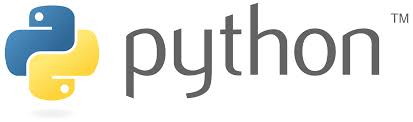
\includegraphics[width=80px]{python}};
%\end{tikzpicture}
\end{frame}

\subsection{Forward Rate Definition}
\begin{frame}{FRA: Forward Rate as Break-Even Rate}
	\begin{block}{Definition}
		The value of $K$ which makes the FRA worth zero is called \textcolor{red}{simply-compounded forward rate}
		\begin{equation}
			F(t;T,S):=\frac{1}{\tau(T,S)}\left[\frac{P(t,T)-P(t,S)}{P(t,S)}\right]
			\label{eq:forward_rate_definition}
		\end{equation}
		The forward rate can be interpreted as a rate observed in $t$ and spanning the time period $S-T$.
	\end{block}
		%Its value depends on no-arbitrage consideration.
	
\end{frame}

\begin{frame}{Forward Rate}
	\begin{itemize}
		\item We can now re-write the value of the FRA in terms of the \emph{simply-compounded forward rate}
		\begin{equation}
			\begin{aligned}
			\textbf{FRA}&=N[\tau KP(t,S)-P(t,T)+P(t,S)] = \\
			&=N\tau P(t,S) \left[K +\frac{1}{\tau} \frac{P(t,S)-P(t,T)}{P(t,S)}\right] = N\tau P(t,S)(K-F(t;T,S))
			\end{aligned}
			\label{eq:fram_payoff_withF}
		\end{equation}
		(\textbf{note:} this formula will be used for the swap evaluation).
		\item<2-> \textcolor{red}{The forward rate can be interpreted as an \emph{estimate} of the future spot rate}, which is unknown at time $t$ (random process based on the market conditions).
	\end{itemize}
\end{frame}

\begin{frame}{Forward Rate}
	Comparing \cref{eq:fram_payoff_withF} to \cref{eq:fra_as_expectation} it is just like we had replaced the IBOR rate $L(T,S)$ with the forward rate $F(t;T,S)$ in the payoff and then taken the present value of the (\emph{now deterministic}) quantity.
	\begin{equation*}
		\begin{aligned}
			\textbf{FRA} &= \mathbb{E}_t[N\tau D(t,S)(K-\overbrace{\textcolor{blue}{F(t; T, S)}}^{\text{replaces } L(T, S)})] = \\
			& = \mathbb{E}_t[N\tau D(t,S)\underbrace{(K-F(t; T, S))}_{\text{deterministic quantity}}] = N\tau P(t,S)(K-F(t; T, S))]
		\end{aligned}
	\end{equation*}
	\emph{We'll see later that indeed $F(t;T,S)$ is the expectation of $L(T,S)$ under a particular probability measure.}
\end{frame}

\begin{frame}{Instantaneous Forward Rate}
	\begin{block}{Definition}
	The \textcolor{red}{instantaneous forward rate} $f(t, T)$ is defined as 
	\begin{equation}
		\begin{aligned}
			f(t, T) &:= \lim_{S\rightarrow T^+} F(t;T,S) =\\
			& = \lim_{\epsilon\rightarrow 0}  \frac{1}{\tau(T,T+\epsilon)}\frac{P(t,T)-P(t,T+\epsilon)}{P(t,T+\epsilon)} = \\
			& = \lim_{\epsilon\rightarrow 0} - \frac{1}{P(t,T)} \frac{P(t,T+\epsilon)-P(t,T)}{\epsilon} =\\
			& = -\frac{\partial \log P(t, T)}{\partial T}
		\end{aligned}
	\end{equation}
\myendproof
	\end{block}
\end{frame}

\begin{frame}{Instantaneous Forward Rate}
	\begin{itemize}
		\item From the previous equation we can derive
		\begin{equation}
			P(t, T) = e^{-\int_t^T f(t, s) ds}
		\end{equation}
		\item The \emph{instantaneous forward rate} represents the rate for a forward contract with an infinitesimal investment period after the settlement date.
		\item Notice that
		\begin{equation*}
			r(t) = f(t,t)
		\end{equation*}
	\end{itemize}
\end{frame}

\begin{frame}[fragile]{FRA: Numerical Example}
A company enters into a FRA to receive 4\% on \$100M for a 3-month period starting in 3 years. Imagine that EURIBOR is 4.5\% in 9 months.
\begin{codebox}
\begin{ipython}[linewidth=\linewidth]
import tensorquant as tq, pandas as pd
from datetime import date, datetime

evaluation_date = tq.Settings.evaluation_date = date(2025, 1, 1)
rates_estr = [0.045, 0.045, 0.045, 0.045]
times_estr = [datetime.strptime(d, "%Y-%m-%d").date() for d in ['2025-04-01', '2028-01-01', '2028-04-01', '2029-01-01']]
market_data = {}
market_data["IR:EUR:ESTR"] = market_data["IR:EUR:3M"] = tq.RateCurve(reference_date=evaluation_date, pillars=times_estr,
                                        rates=rates_estr, interp='LINEAR',  daycounter_convention=tq.DayCounterConvention.ActualActual)
eur3m_index = tq.IborIndex(calendar, 3, tq.TimeUnit.Months, tq.Currency.EUR, 2)
eur3m_index.add_fixing(evaluation_date, 0.045)

notional=100e6
fixed_rate = 0.04
eur_fra_builder = tq.FraGenerator(ccy=tq.Currency.EUR, start_delay=2, fixing_days=2, index_term="3M", 
                                  roll_convention= tq.BusinessDayConvention.ModifiedFollowing, notional=notional,
                                  day_count_convention=tq.DayCounterConvention.Actual360, calendar=tq.TARGET(), index=eur3m_index)
fra = eur_fra_builder.build(trade_date=evaluation_date, quote=fixed_rate, term="3M-12M")
fra_engine = tq.FraPricer(tq.market_map)
fra_engine.price(fra, market_data, True)
print(f"NPV FRA: {fra.price :,.0f}")
\end{ipython}
\begin{ioutput}
NPV FRA: 329,145
\end{ioutput}
\end{codebox}
\end{frame}

\begin{homework}
\begin{frame}{\textcolor{white}{Homework}}
\begin{itemize}
	\item[white] A $3\times 9$ Forward Rate agreement refers to:
		\begin{itemize}
			\item[white] a 90-day LIBOR loan starting 270 days from now;
			\item[white] a 270-day LIBOR loan starting 90 days from now;
			\item[white] a 180-day LIBOR loan starting 90 days from now.
		\end{itemize}
	\item[white] Suppose we have a $1\times 4$ FRA with a notional principal of €1 million.  At contract expiration, the 90-day LIBOR at settlement is 6\% and the contract rate is 5.5\%. Calculate the value of the FRA at maturity.
	\item[white] The 1-year spot rate on US treasury bonds is 9\%, the 2-year spot rate is 9.5\% and the 3-year spot rate is 10\%. 
	\begin{itemize}
		\item[white] Calculate the implied 1-year ahead, 1-year forward rate, $F(0;1,2)$. Explain why a 1-year forward rate of 9.6\% could not be explained by the market;
		\item[white] calculate the forward rates  $F(0; 2, 3)$ and $F(0; 1,3)$. Is there a link between $F(0;1,2),F(0;2,3)$ and $F(0;1,3)$ ?
	\end{itemize}
\end{itemize}
\end{frame}
\end{homework}

\section{Interest Rate Swap}
\begin{frame}{Interest Rate Swap}
	\begin{itemize}
		\item An \textcolor{red}{Interest Rate Swap} (IRS) is a contract that exchanges payments between two differently indexed \emph{legs}, starting from a future time. At every pre-specified instant $T_i$, the \emph{fixed leg} pays the amount ($N$ is the contract nominal)
		\begin{equation*}
			C_{\text{fixed}} = N\tau(T_{i-1}, T_i)K
		\end{equation*}
		while the \emph{variable leg} pays the amount
		\begin{equation*}
			C_{\text{floating}} = N\tau(T_{i-1}, T_i)L(T_{i-1}, T_i)
		\end{equation*}
		where for simplicity we are assuming the same payment dates for the two legs.
		\item<2-> When the fixed leg is paid, the IRS is termed \textcolor{red}{Payer IRS}. If the opposite holds, we have a \textcolor{red}{Receiver IRS}.
		\item<3-> The discounted payoff of a \emph{Payer IRS} can be expressed as:
		\begin{equation}
			N\sum_{i=\alpha+1}^{\beta} D(t,T_i) \underbrace{\tau_i}_{\tau(T_{i-1},T_i)}
			\left[L(T_{i-1},T_i)-K\right]
			\label{eq:payoff_payer_irs}
		\end{equation}	
	\end{itemize}
\end{frame}

\begin{frame}{Interest Rate Swap}
\begin{center}
	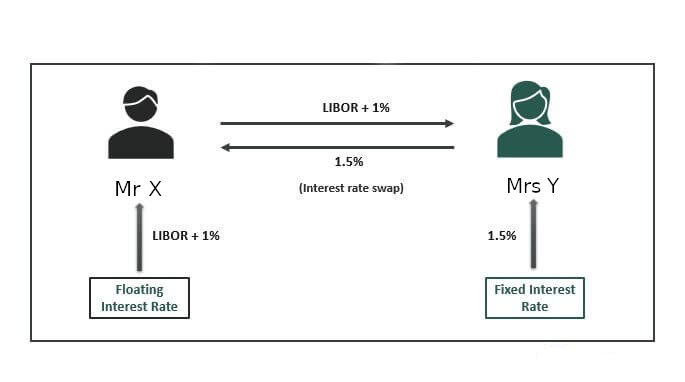
\includegraphics[width=0.9\linewidth]{images/Interest-Rate-Swap-diagram}
\end{center}
\end{frame}

\begin{frame}{IRS and FRA}
	\begin{itemize}
		\item The swap payoff in \cref{eq:payoff_payer_irs} can be re-interpreted as a portfolio of FRAs.
		\item Indeed consider a \emph{Receiver IRS} and express its payoff as a sum of FRAs using \cref{eq:fram_payoff_withF}
		\begin{equation*}
			\begin{aligned}
				\textbf{RFS}&(t,T,\tau,N,K) = N\sum_{i=\alpha+1}^{\beta}\expect{Q}[D(t,S)\tau_i(K - L(T_{i-1},T_i))]=\\
				&=N\sum_{i=\alpha+1}^{\beta}\tau_i P(t,T_i)(K-F(t;T_{i-1},T_i))=\\
				&=N\sum_{i=\alpha+1}^{\beta}\tau_i KP_i-N\sum_{i=\alpha+1}^{\beta}(P_{i-1}-P_i)=\quad (\text{where }P(t, T_i) = P_i) \\
				&=N\sum_{i=\alpha+1}^{\beta}\tau_i KP_i-N[(P_\alpha -\cancel{P_{\alpha+1}}) + (\cancel{P_{\alpha+1}} - \cancel{P_{\alpha+2}}) + \ldots + (\cancel{P_{\beta-1}} - P_{\beta})] \\
			\end{aligned}
		\end{equation*}
	\end{itemize}
\end{frame}

\begin{frame}{IRS and FRA}
	\begin{itemize}
		\item The swap payoff in \cref{eq:payoff_payer_irs} can be re-interpreted as a portfolio of FRAs.
		\item Indeed consider a \emph{Receiver IRS} and express its payoff as a sum of FRAs using \cref{eq:fram_payoff_withF}
		\begin{equation}
			\begin{aligned}
				\textbf{RFS}&(t,T,\tau,N,K) = 	N\sum_{i=\alpha+1}^{\beta}\expect{Q}[D(t,S)\tau_i(K - L(T_{i-1},T_i))]= \ldots =\\
				&=N\sum_{i=\alpha+1}^{\beta}\tau_i KP_i-N[(P_\alpha -\cancel{P_{\alpha+1}}) + (\cancel{P_{\alpha+1}} - \cancel{P_{\alpha+2}}) + \ldots + (\cancel{P_{\beta-1}} - P_{\beta})] =\\
                &=\boxed{N\sum_{i=\alpha+1}^{\beta}\tau_i KP(t,T_i)-NP(t,T_\alpha)+NP(t,T_\beta)}\quad\quad\quad\qedsymbol
			\end{aligned}
		\label{eq:swap_as_sum_fra}
		\end{equation}
	\end{itemize}
\end{frame}

\begin{frame}{IRS and FRA}
	\begin{itemize}
		\item<1-> Even if a swap at inception has a null NPV, not all the FRAs in a swap with zero value have zero value (\emph{except for the degenerate case of flat yield curve}): some of them will have positive NPV, some other negative; the only constraint being their sum to be zero.
		\item<2-> In a \emph{Payer Swap} with an increasing yield curve the first FRAs will have negative value, the last positive. Still their NPV's sum is zero.
		\item<3-> If the market doesn't move so much the swap rate payer will have to pay a net interest differential in the first part of the contract life, and to receive net interest in the second.
		\item<4-> So the rate payer will have to fund the payments for the first part of the contract and to invest at his best the receipt during the second part. (this feature is sometimes referred to as the \emph{funding profile of the contract}).
	\end{itemize}
\end{frame}

\begin{frame}[fragile]{IRS as FRA Example}
\begin{columns}
    \column{0.65\linewidth}
\begin{ipython}
from datetime import date
from dateutil.relativedelta import relativedelta

def makePFS(rates):
  vals = []
  today = date.today()
  dfs = [1/(1+rates[i])**i for i in range(1, len(rates))]
  dc = DiscountCurve(today,
                     [today+relativedelta(years=i) for i in range(1, len(rates))],
                     dfs)
  dummy_irs = InterestRateSwap(1, today, "5y", 0.137, "1y", side=SwapSide.Payer)
  swap_rate = dummy_irs.swap_rate(dc)
  irs = InterestRateSwap(1, today, "5y", swap_rate, "1y", side=SwapSide.Payer)
  val, vals = irs.npv_with_FRA(dc)

makePFS([0.05, 0.07, 0.09, 0.11, 0.13, 0.15, 0.17])
makePFS([0.05] * 7)
makePFS(list(reversed([0.05, 0.07, 0.09, 0.11, 0.13, 0.15, 0.17])))
\end{ipython}
    \column{0.35\linewidth}
    %\begin{center}
        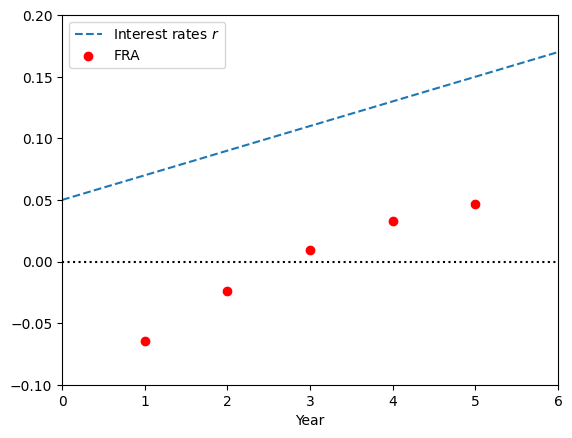
\includegraphics[width=0.62\linewidth]{images/swap_fra_up.png}\\
        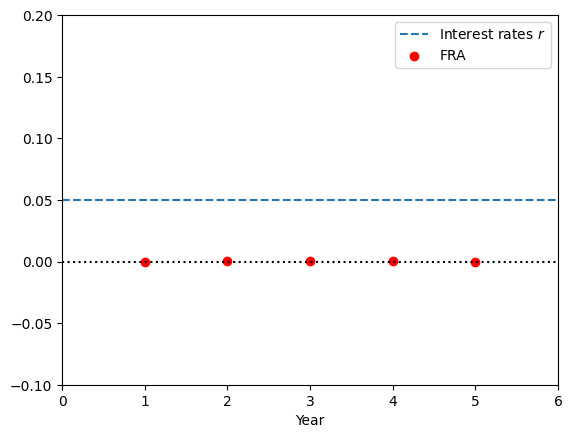
\includegraphics[width=0.62\linewidth]{images/swap_fra_flat.png}\\
        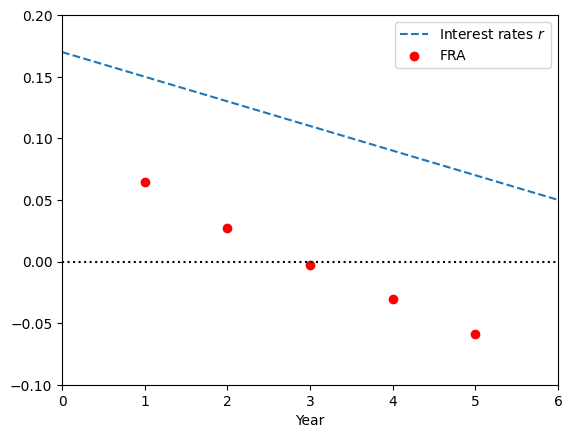
\includegraphics[width=0.62\linewidth]{images/swap_fra_down.png}\\
    %\end{center}
\end{columns}
    
\end{frame}

\begin{homework}
\begin{frame}{\textcolor{white}{Homework}}
\begin{itemize}
\item[white] Assume that company A has agreed to pay a 6-month Libor and receive a fixed interest rate of 8\% per annum (with interest payable every six months) from the face value of 100 million. Swap is 1.25 years to expire. The interest rates for 3, 9 and 15 months are: 10\%, 10.5\% and 11\% respectively. Assume that interest rates are continously compounded. The 6-month Libor is currently 10.2\%. Calculate the value of this swap for company A. Determine the value of the swap using the relationship between interest rate swap and FRA.
\item[white] Which of the following strategies is (are) appropriate ?
\small{
\begin{itemize}
	\item[white] If a borrower has a fixed rate debt and is expecting interest rates to rise, then the borrower should not enter into a swap.
	\item[white] If an investor has floating rate assets and is expecting interest rates to rise, then the investor should enter into a receiver swap.
	\item[white] If a borrower has floating rate debt and is expecting interest rates to rise, then the borrower should enter into a payer swap.
	\item[white] If an investor has fixed income assets and is expecting interest rates to drop, then the investor should enter into a payer swap.
\end{itemize}}
\end{itemize}
\end{frame}
\end{homework}

\subsection{Swap Rate}
\begin{frame}{Swap Rate as Break-Even Rate}
	Similarly to FRA break-even rate\ldots
	\begin{block}{Definition}
	The fixed rate $K$ which makes the above expression null is called \textcolor{red}{forward swap rate}:
	\begin{equation}
		S_{\alpha,\beta}(0) = \frac{P(0, T_\alpha)-P(0,T_\beta)}{\sum_{i=\alpha+1}^{\beta}\tau_iP(0,T_i)}
	\end{equation}
	If $T_\alpha=0$ we have the \textcolor{red}{spot swap rate} (which is published on financial newspapers).
	\end{block}
	The swap rate makes the contract fair at inception by definition.
\end{frame}

\begin{frame}{Swap Payoff Alternative Expression}
	\begin{itemize}
		\item<1-> Consider a Payer IRS with $N=1$ for simplicity (using \cref{eq:swap_as_sum_fra})
		\begin{equation*}
			\textbf{PFS} = P(t,T_\alpha)-P(t,T_\beta)-\sum_{i=\alpha+1}^{\beta}\tau_iKP(t,T_i)
		\end{equation*}
		\item<2-> By multiplying and dividing by (the so called \textcolor{red}{annuity}) $A = \sum_{i=\alpha+1}^{\beta}\tau_i P(t, T_i)$
		we get
		\begin{equation}
			\begin{gathered}
			\textbf{PFS}=\frac{A}{\sum\tau_iP(t, T_i)}\left[P(t,T_\alpha)-P(t,T_\beta)-K\sum_{i=\alpha+1}^{\beta}\tau_i P(t,T_i)\right]=\\
			= \boxed{A (S_{\alpha,\beta}(t)-K)}
			\end{gathered}
		\label{eq:swap_payoff_with_swap_rate}
		\end{equation}
		(\textbf{note:} this expression will be useful when pricing swaptions).
	\end{itemize}
\end{frame}

\begin{frame}{Swap Curve}
\begin{itemize}
	\item The \emph{swap curve} is a graphical representation of the relationship between the fixed interest rate and the maturity of IRS (typically ranging from 1 to 30 years).
	\item These swap rates are determined through market transactions, reflecting the market's consensus on future interest rate expectations.
	\begin{columns}
		\column{0.35\linewidth}
		\begin{center}
			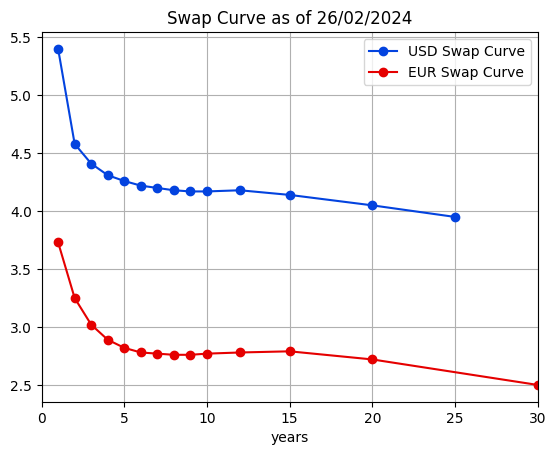
\includegraphics[width=1\linewidth]{images/swap_curve}
		\end{center}
		\column{0.65\linewidth}
		\small{
		\item An upward-sloping \emph{(normal)} curve indicates longer-term interest rates are higher than short-term rates (expectations of economic growth and inflation). 
		\item A downward-sloping \emph{(inverted)} curve suggests short-term rates are higher than long-term rates (potential economic downturns or market uncertainties).}
		%\item A flat curve indicates that short and long-term rates are relatively similar, indicating a neutral market sentiment.}
	\end{columns}
	\item Swap rates are often used as benchmarks for pricing other financial instruments, such as corporate bonds and loans.
\end{itemize} 
\end{frame}

\begin{frame}{Yield vs Swap Curve} 
\begin{itemize}
\item Several factors can impact swap curve movements (changes in interest rates, market sentiment, economic indicators, and central bank policies).
\item One way to interpret it is to make a comparison with the yield curve.
\item Since the swap curve reflects exchanged rates over various time horizons, it offers a more accurate representation of market expectations and risk perceptions, as it is based on actual transactions.
\begin{columns}
\column{0.65\linewidth}
\item It essentially shows how much more (or less) it costs to pay a fixed rate in a swap compared to lending to the government.
\item The shape of the swap spread curve can provide insights into market expectations about future interest rates and economic conditions.
\item Swap spreads reflect the perceived credit risk of banks relative to the government. Wider spreads may indicate concerns about bank health. 
\column{0.35\linewidth}
\begin{center}
	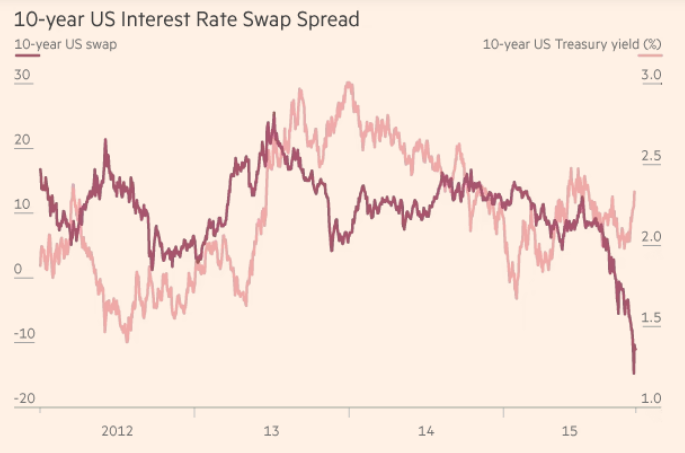
\includegraphics[width=1.\linewidth]{images/swap_spread}
\end{center}
\end{columns}
\end{itemize}
\end{frame}

\begin{frame}{Trading and Hedging Strategies}
\begin{itemize}
\item Suppose that there is an unexpected increase in inflation expectations due to rising commodity prices. This change would likely cause the swap curve to shift upward, reflecting the higher expected future interest rates. 
\item Market participants who anticipate this shift may adjust their swap positions accordingly, either by entering into longer-term swaps or adjusting the mix of fixed and floating rates in their portfolios.
\item When evaluating the swap curve, market participants should compare the benefits and drawbacks of floating and fixed rates. 
\item Floating rates (such as those linked to LIBOR or EURIBOR), can provide flexibility and potentially lower costs, as they reflect the prevailing market conditions. 
\item On the other hand, fixed rates offer certainty and protection against potential interest rate hikes. 
\end{itemize}
\end{frame}

\begin{frame}{Trading and Hedging Strategies}
\begin{itemize}
\item Market participants need to carefully assess their risk appetite and market expectations to determine the most suitable rate structure for their swap transactions.
\item From the perspective of a fixed-rate receiver, the swap curve determines the level of fixed interest payments they will receive over the life of the swap. 
\item If the swap curve is upward sloping, the receiver would demand a higher fixed rate to compensate for the expected rise in interest rates. 
\item Conversely, if the swap curve is downward sloping, it suggests that market expectations for future interest rates are declining, and a fixed-rate receiver would be willing to accept a lower fixed rate.
\end{itemize}
\end{frame}

\begin{frame}{Trading and Hedging Strategies}
	\begin{itemize}
		\item With a Swap you can have a clear picture of the market. For example if you own the $5y$, you make money if rates go higher, loose money if they go lower.
		\item With two Swaps instead you can bet on the \textcolor{red}{slope} of the interest rate curve.
		\item If you bet on steepening of the $30y-10y$ slope, you pay the $10y-30y$; if you bet on flattening on the same portion of the yield curve you receive the $10y-30y$.		
		%\item With Swaps you can bet on the \emph{bund basis}: this quantity is linked to the evolution of credit and liquidity in the inter-bank and Government bond markets.
	\end{itemize}
\end{frame}

%1. Diversification: One of the most fundamental strategies for managing swap curve risks is diversification. By spreading investments across different points on the swap curve, investors can reduce their exposure to specific interest rate changes. For example, if an investor holds a portfolio of plain vanilla swaps with varying maturities, they are less vulnerable to sudden shifts in the swap curve at a particular point in time. Diversification allows for a balanced risk exposure and can help protect against adverse market conditions.

%2. Hedging: Hedging is another strategy commonly used to manage swap curve risks. By entering into offsetting positions, investors can protect themselves from potential losses due to changes in the swap curve. For instance, if an investor holds a long position in a plain vanilla swap, they can hedge their risk by taking a short position in another swap with similar characteristics but at a different point on the swap curve. This way, any adverse movement in the swap curve would be offset by gains in the hedging position.

%3. Dynamic Positioning: Instead of maintaining a static portfolio of plain vanilla swaps, some investors opt for dynamic positioning. This strategy involves actively adjusting the positions in response to changes in the swap curve. By closely monitoring the swap curve and making timely adjustments, investors can take advantage of favorable movements and minimize the impact of adverse shifts. For example, if the swap curve steepens, an investor may choose to increase their exposure to longer-dated swaps to capture higher yields.

%4. duration matching: Duration matching is a strategy that aims to minimize interest rate risk by aligning the duration of a plain vanilla swap with the investor's investment horizon. Duration represents the weighted average time to receive or pay cash flows from a swap. By matching the duration of the swap with the investment horizon, investors can reduce the impact of changes in the swap curve on their portfolio's value. This strategy is particularly useful for risk-averse investors who prioritize stability and predictability.

\subsection{Swap and Bond Switching}
\begin{frame}{Swap and Bond Switching}
	\begin{itemize}
		\item<1-> Consider again a Payer Forward Swap (this time with notional $N$)
		\begin{equation*}
			\textbf{PFS}(t,T_\alpha,T_\beta,\tau,N,K)=N(P(t,T_\alpha)-P(t,T_\beta))-NK\sum_{i=\alpha+1}^{\beta} \tau_iP(t,T_i)
		\end{equation*}
		\item<2-> A swap can be considered as an exchange between two kinds of bond with the same notional reimbursed at maturity. In fact:
		\begin{itemize}
		 \item<3->\emph{the fixed leg} of the swap can be viewed as a \textcolor{red}{fixed coupon stream};
		 \item<3-> while the \emph{variable} can be considered a \textcolor{red}{floating rate note coupon stream}. 
		\end{itemize}
	\end{itemize}
\end{frame}

\begin{frame}{Fixed Rate Side}
	\begin{itemize}
		\item<1-> Consider a coupon bond that pays the following cash flows $\mathcal{C}=\{c_{\alpha+1},\ldots,c_\beta\}$ on the schedule $\mathcal{T} = \{T_{\alpha+1},\ldots,T_\beta\}$ with 
		\begin{equation*}
			\begin{cases}
				c_i = N\tau K,\quad i<\beta \\
				c_\beta=N\tau K+N, \quad i=\beta	
			\end{cases}		
		\end{equation*}
		\item<2-> The coupon bond price can be written as the discounted sum of the cash-flows
		\begin{equation}
			\textbf{CBP}(t,\mathcal{C},T)=\sum_{i=\alpha+1}^{\beta}c_i P(t,T_i)
		\end{equation}
		\item<3-> Needless to say that in case $K=0$ the bond reduces to a zero-coupon bond with maturity $T_\beta$.
		
%		\item Last equation rearranged gives
%		\begin{equation}
%			\textbf{CBP}(t,T_\beta,K,N) = N - PS(t,T_\beta)
%		\end{equation}
	\end{itemize}
%	\begin{block}{Intepretation}
%		The meaning is pretty straightforward: a fixed rate bond can be replicated using the NPV of a payer swap whose fixed leg coincides with the fixed leg of the bond. The floating leg represents the funding of the bond, i.e. the interests the issuer must pay to raise funds in the interbank market when his spread over the benchmark LIBOR rate is null.
%	\end{block}
\end{frame}

%\begin{frame}{Swap and Bond Switching}
%	\begin{itemize}
%		\item More formally, consider a coupon bond that pays the following cash flows $\mathcal{C}=[c_{\alpha+1},\ldots,c_\beta]$	on the schedule $T = [T_{\alpha+1},\ldots,T_\beta]$ with 
%		\begin{equation*}
%			\begin{cases}
%			c_i = N\tau K,\quad i<\beta \\
%			c_\beta=N\tau K+N, \quad i=\beta	
%			\end{cases}		
%		\end{equation*}
%		\item The coupon bond price can be written as
%		\begin{equation}
%			\textbf{CBP}(t,\mathcal{C},T)=\sum_{i=\alpha+1}^{\beta}c_i P(t,T_i)
%		\end{equation}
%	\end{itemize}
%\end{frame}

\begin{frame}{Floating Rate Note (FRN)}
	\begin{itemize}
		\item<0-> Next consider a floating rate note that pays coupons at dates
		\begin{equation*}
			\mathcal{T}_{\text{payments}} = \{T_{\alpha+1},\ldots,T_\beta\}
		\end{equation*}
		coupons calculated at the EURIBOR rate fixed in the previous period
		\begin{equation*}
			\mathcal{T}_{\text{fixings}} = \{T_{\alpha},\ldots,T_{\beta - 1}\}
		\end{equation*}
		\item<1-> At maturity $T_\beta$ the notional is reimbursed as before.
		\item<2-> To value this note we change sign to the \textbf{RFS} (\cref{eq:swap_as_sum_fra}), set $K=0$, i.e. no fixed rate payments are done, and finally add the present value of the notional at maturity: $NP(t,T_\beta)$
		\begin{equation*}
			\begin{aligned}
			\textbf{FRN} &= -\textbf{RFS} + NP(t,T_\beta) =\\
			& =NP(t,T_\alpha)-NP(t,T_\beta)-N\sum_{i=\alpha+1}^{\beta}K\tau_i P(t,T_i) + NP(t,T_\beta)
		\end{aligned}
		\end{equation*}
	\end{itemize}
\end{frame}

\begin{frame}{Floating Rate Note (FRN)}
	\begin{itemize}
		\item Next consider a floating rate note that pays coupons at dates
		\begin{equation*}
			\mathcal{T}_{\text{payments}} = \{T_{\alpha+1},\ldots,T_\beta\}
		\end{equation*}
		coupons calculated at the LIBOR rate fixed in the previous period
		\begin{equation*}
			\mathcal{T}_{\text{fixings}} = \{T_{\alpha},\ldots,T_{\beta - 1}\}
		\end{equation*}
		\item At maturity $T_\beta$ the notional is reimbursed as before.
		\item To value this note we change sign to the \textbf{RFS} (\cref{eq:swap_as_sum_fra}), set $K=0$, i.e. no fixed rate payments are done, and finally add the present value of the notional at maturity: $NP(t,T_\beta)$
		\begin{equation*}
		\begin{aligned}
			\textbf{FRN} &= -\textbf{RFS} + NP(t,T_\beta) =\\
			& =NP(t,T_\alpha)-\cancel{NP(t,T_\beta)}-\cancel{N\sum_{i=\alpha+1}^{\beta}K\tau_i P(t,T_i)} + \cancel{NP(t,T_\beta)} =NP(t,T_\alpha)
		\end{aligned}
		\end{equation*}
	\end{itemize}
\end{frame}

\begin{frame}{Floating Rate Note (FRN)}
	\begin{itemize}
	\item The intuition behind this formula is quite straightforward: if we set $T_\alpha =t$. 
	\begin{equation*}
		\textbf{FRN} = N P(t, T_\alpha) = N P(t, t) = N
	\end{equation*}
	\textcolor{red}{At the date of the first reset, the bond price equals par.} 
	\item This result also holds for all the dates equal to the reset of the floating rates (an \textbf{FRN} is equivalent to a roll-over strategy of short-term loans).
	\item This property is sometimes summarized by the sentence \emph{"the \textbf{FRN} always trade at par"}.
	\item The \textbf{FRN} is a debt security in which coupon payments adjust according to changes in interest rates. The coupons are closely tied to current short-term spot rates, such that their prices are always at or near par value (no arbitrage). 
	%\item Provide an example of Italian government floating rate note. Did they trade at par in recent times ? Provide an explanation.
	\end{itemize}
\end{frame}

\begin{frame}{Floating Rate Note Example}
\begin{itemize}
\item Floating rate bond (FRN) usually refers to an instrument whose coupon is based on a short term rate (3-month T-bill, 6-month EURIBOR). 
\item Variable coupon rates are fixed in advance at reset dates, which are 3- or 6-month (interest payment period) earlier.
\item FRN price (with \emph{unit notional amount}), $n$ maturity, annual frequency ($\tau=1$), and the first coupon rate pre-determined at previous reset date ($C_{reset}$) is as follows:

\begin{equation*}
\begin{aligned}
\textbf{FRN} & = D_{0,1}C_{reset} + \sum_{i=1}^nD_{0,i+1}F_{i,i+1} + D_{0,n}= \\
& = D_{0,1}C_{reset} + D_{0,2}F_{1,2} + \ldots + D_{0,n-1}F_{n-2,n-1}+ D_{0,n}(1+F_{n-1,n}) = \\
& = D_{0,1}C_{reset} + D_{0,2}\left(\frac{D_{0,1}}{D_{0,2}}-1\right) + \ldots + D_{0,n}\left(\frac{D_{0,n-1}}{D_{0,n}}-1\right) + D_{0,n} = \\
\end{aligned}
\end{equation*}
where $f(t_1,t_2)$ denotes the forward rate between $t_1$ and $t_2$.
\end{itemize}
\end{frame}

\begin{frame}{Floating Rate Note Example}
\begin{equation*}
\begin{aligned}
\textbf{FRN} & = D_{0,1}C_{reset} + (D_{0,1} - D_{0,2}) +(D_{0,2} - D_{0,3}) + \ldots + \\
& + (D_{0,n-2} - D_{0,n-1}) + (D_{0,n-1} - D_{0,n}) + D_{0,n} = \\
& = \boxed{D_{0,1} (1 +C_{reset})}
\end{aligned}
\end{equation*}
\begin{itemize}
\item The price of FRN has a range from \emph{par to par} + full coupon. It is par right before the reset date and is C right after the reset date (and is linear when pricing date is between two reset dates).
\item Draw a plot showing the characteristic sawtooth behaviour of a floating rate note. 
\begin{equation*}
\textbf{FRN} = D_{0,1}C_{reset} + \sum_{i=1}^nD_{0,i+1}F_{i,i+1} + D_{0,n}
\end{equation*}
\end{itemize}
\end{frame}

\begin{frame}[fragile]{Floating Rate Note Example}
\begin{columns}
\column{0.5\linewidth}
\begin{ipython}
import pandas as pd, numpy as np

from datetime import date
from dateutil.relativedelta import relativedelta

frn = FloatingRateNote(date.today(), "3Y", "3m")
pillars = [date.today()+relativedelta(months=dt_from_str(f"{t}M")) 
           for t in rates['T']]
rates = rates['r'].values
prices = []

d = date.today()
for i in range(0, 367*2):
  next_pillars = [p for p in pillars if p >= d]
  dts = [(p-d).days/360 for p in next_pillars]
  dfs = [np.exp(-dt*rates[i]) for i, dt in enumerate(dts)]
  dc = DiscountCurve(d, next_pillars, dfs)

  prices.append(frn.price(d, dc))
  d = date.today()+relativedelta(days=i)
\end{ipython}
\column{0.5\linewidth}
\begin{center}
    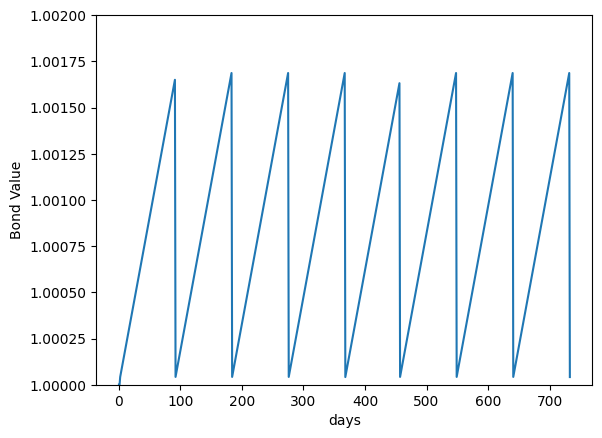
\includegraphics[width=0.9\linewidth]{images/frn_sawtooth}
\end{center}
\end{columns}
\end{frame}

\subsection{Fixed vs Variables}
\begin{frame}{Concepts behind the Formulas}
	Suppose that a generic bank, \emph{MyFavouriteBank}, has the same credit risk of the corresponding average inter-bank entity. So, \textcolor{red}{the spread over the EURIBOR rate is 0}. Suppose now the bank needs financing and it plans to issue coupon bonds. It has two alternatives:
	\begin{enumerate}
		\item<1-> borrow $N$ and pay floating interests at the rates
		\begin{equation*}
			L(T_{i-1},T_i);
		\end{equation*}
		\item<1-> borrow $N$ and pay fixed interests given by the coupon
		\begin{equation*}
			K = S_{\alpha,\beta}.
		\end{equation*}
		(clearly the overall cost to raise money must be the same at the beginning, i.e. fixed leg NPV equals floating leg NPV).
	\end{enumerate}
\end{frame}

\begin{frame}{Concepts behind the Formulas}
	\begin{itemize}
		\item<1-> Given the two strategies are equivalent the bank will then opt for one of two alternatives depending on:
		\begin{enumerate}
			\item marketing considerations, i.e. which kind of bond people prefer;
			\item the interest rate risk it wants to have.
		\end{enumerate} 
		\item<2-> Remember that a variable rate mortgage is perceived risky by the average individual as salary is more or less fixed, but for bank this is not the case because it is left unarmed by the rate rise. Indeed if rates go up
		\begin{itemize}
			\item the bank loses in the higher coupons it has to pay to the bond holders;
			\item the bank gains in the higher rates it charges on new loans at the same time.
		\end{itemize}
		\item<3-> This is the most basic example of \emph{asset liability matching}.
		\item<3-> The same more or less holds for a rate decrease.%, but with some caveats.
	\end{itemize}
\end{frame}

\begin{frame}{Concepts behind the Formulas}
	\begin{itemize}
		\item<0->Although banks like more floating rates exposure, there are pros and cons for this choice: 
		\begin{itemize}
			\item<1-> [\goodcheck] the liability value (the bond floating rate) resets with rates;
			\item<1-> [\goodcheck] often the costs are smaller then fixed rates;
			\item<1-> [\goodcheck]surely less expensive in the case of a long-term loan (e.g. 30-year mortgage), lenders require higher fixed rates in that case, due to bad accuracy in forecast economic conditions over such a long period of time.
		%\end{itemize}
		%\begin{itemize}
			\item<2-> [\badcheck] higher interest rate risk (risk of rising rates in the future);
			\item<2-> [\badcheck] with inverted yield curve, the cost of debt may actually be higher than fixed-rate. They have to offer higher interest rates to attract buyers, especially for long-term debt. since investors are demanding more compensation for the perceived economic slowdown risk (however, this is the exception rather than the norm).
		\end{itemize}
% There is a general assumption that interest rates will rise – or, increase – over time,
		\item<3-> So why do not banks issue only floating rate notes ?
		\item<4-> Banks must issue fixed rate coupon bonds to attract customers (think of yourself or insurance companies) but then will hedge the liability  with an investment bank. In this way the final risk exposure will be at a variable rate as they like. 
		%\item<3-> \textcolor{red}{Swaps are both a hedging instrument and a pricing tool.}
	\end{itemize}
\end{frame}

%\begin{frame}{Concepts behind the Formulas}
%	\begin{itemize}
%		\item<1-> So why do not banks issue only floating rate notes ?
%		\item<2-> Banks must issue fixed rate coupon bonds to attract customers (think of yourself or insurance companies) but then will hedge the liability  with an investment bank. In this way the final risk exposure will be at a variable rate as they like. 
%		\item<3-> \textcolor{red}{Swaps are both a hedging instrument and a pricing tool.}
%	\end{itemize}
%\end{frame}

\subsection{Basis Swaps}
\begin{frame}{Basis Swap}
	\begin{itemize}
	\item A \textcolor{red}{(Tenor) Basis Swap} is defined as a contract in which two floating legs are exchanged.
	\item The two legs can differ both in the tenor of the underlying rate and in the frequency of payments.
	\item For instance a typical Basis Swap is one in which a floating leg indexed to EURIBOR-6M is exchanged against one indexed to EURIBOR-3M.
	\end{itemize}
	\begin{center}
		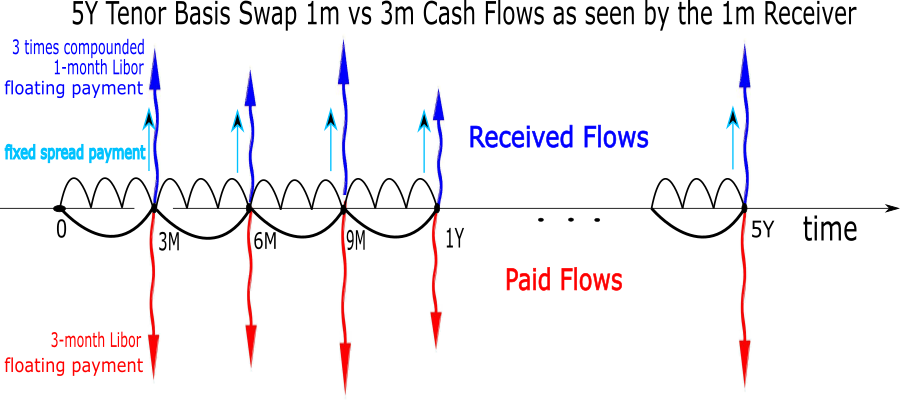
\includegraphics[width=0.6\linewidth]{images/tenor_basis_swap}
	\end{center}
\end{frame}

\begin{frame}{Basis Swap Valuation}
\begin{itemize}
	\only<1-2>{
	\item A Tenor Basis Swap can be priced according to the following expression
	\begin{equation}
	\boxed{
		\begin{aligned}
			\textbf{TBS}(t) = \sum_{i=1}^n \tau_i^{L} F^{L}&(t;T_{i-1},T_i)P(t,T_i) - \\
			&- \sum_{j=1}^m \tau_j^{S} (F^{S}(t;T_{j-1},T_j)+s)P(t,T_j)
		\end{aligned}
	}
	\end{equation}
	where $L$ (long index) denotes the index with the longer tenor and $S$ (short index) the other with the shorter tenor.}
	\only<3->{
	\item A Tenor Basis Swap can be priced according to the following expression
	\begin{equation}
	\boxed{
	\begin{aligned}\textbf{TBS}(t) = \sum_{i=1}^n \tau_i^{L} F^{L}&(t;T_{i-1},T_i)P(t,T_i) - \\
	&-\sum_{j=1}^m \tau_j^{S} (F^{S}(t;T_{j-1},T_j)+\textcolor{red}{s})P(t,T_j)
	\end{aligned}
	}
	\end{equation}
	where $L$ (long index) denotes the index with the longer tenor and $S$ (short index) the other with the shorter tenor.}

	\item<2-> Basis Swaps usually quote at par, meaning that the price of the swap is zero and that the present value (PV) of each of the traded legs is the same. 
	\item<3-> This is made possible by adding a \textcolor{red}{basis spread $s$} to the LIBOR index with the lower frequency tenor.
	\end{itemize}
\end{frame}

\begin{frame}{Basis Swap Spread}
	\begin{itemize}
	\item But according to the \textcolor{red}{single curve framework} there should be no basis as the value of the floating leg is given by (assuming $N=1$)
	\begin{equation*}
	P(0, T_0) - P(0, T_n), \quad \text{(forward start case)}
	\end{equation*}
	or by 
	\begin{equation*}
	1 - P(0, T_n), \quad \text{(spot case)}
	\end{equation*}
	\begin{columns}
	\column{0.4\linewidth}
	\item In both cases what matters are the first and the last payment dates; hence if they are the same for the two legs (regardless the reset frequency and the index tenor), the basis should be zero.
	\column{0.4\linewidth}
		\begin{center}
		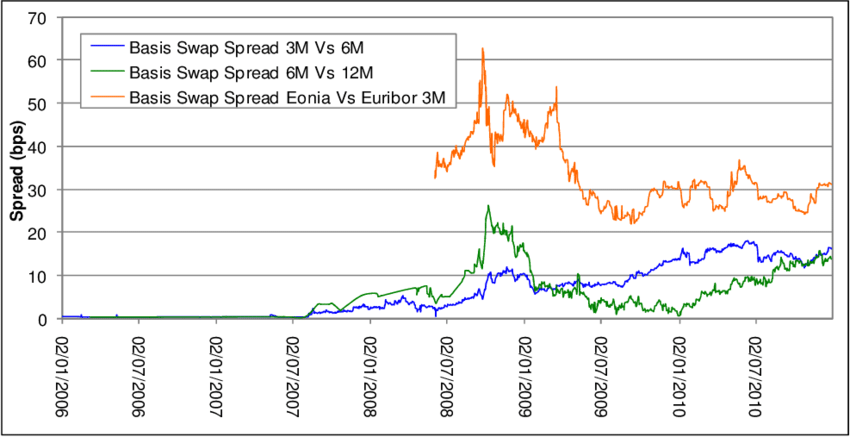
\includegraphics[width=1.1\linewidth]{images/Basis-Swap-spreads-Euribor-3M-Vs-Euribor-6M-Euribor-6M-Vs-Euribor-12M-and-Eonia-Vs}
		\end{center}
	\end{columns}
	\end{itemize}
	%Exercise: write in detail the above argument, and provide an example for both a 10Y spot start basis swap and a 1Y forward 10Y Swap. Which condition you need to derive the result?
\end{frame}

\section{Credit Risk and Asset Swap}
\begin{frame}{Adding Credit Risk}
	\begin{itemize}
		\item When we make the real world enter the picture, a typical bank will pay a spread over EURIBOR representing the \textcolor{red}{credit risk} (and other stuff, but leave this extra aside here). 
		%\item For the swap to be worth 0 at inception the fixed rate must be higher as well. 
		\item<2-> Hence a bank, which \emph{has credit risk},  will have to pay
		\begin{enumerate}
			\item a higher coupon if it issues a bond with fixed coupon;
			\item a spread over the variable rate if it opts for a floating rate bond.
		\end{enumerate}
		\item<3-> Often, in the first case, it will swap the liability, i.e. the bank is liable towards the bond holders, to hedge the pure rate risk. 
		\item<4-> This lead us to the next topic, the Asset Swap contract.
	\end{itemize}
\end{frame}

\begin{frame}{Par Asset Swap}
	\begin{itemize}
		\item<1-> An \textcolor{red}{Asset Swap} (AS) can be defined as a \emph{synthetic floating-rate note}.
		\item In fact, the Asset Swap transforms a fixed rate into a floating one, \textcolor{red}{leaving the credit risk profile unchanged}.
		\item<1-> There are several kinds of Asset Swap contract, in the following we are going to consider \textcolor{red}{Par Asset Swaps}. 
		\item<2-> The package is made of a position in a bond and another in a swap.
		\item<3-> In case of \textbf{default} of the bond issuer, the Asset Swap buyer \textbf{must pay the fixed leg and the principal in the swap} but \textcolor{red}{does not receive the coupon} of the defaulted bond. 
	\end{itemize}
\end{frame}

\begin{frame}{Valuation of the Asset Swap}
	\begin{center}
		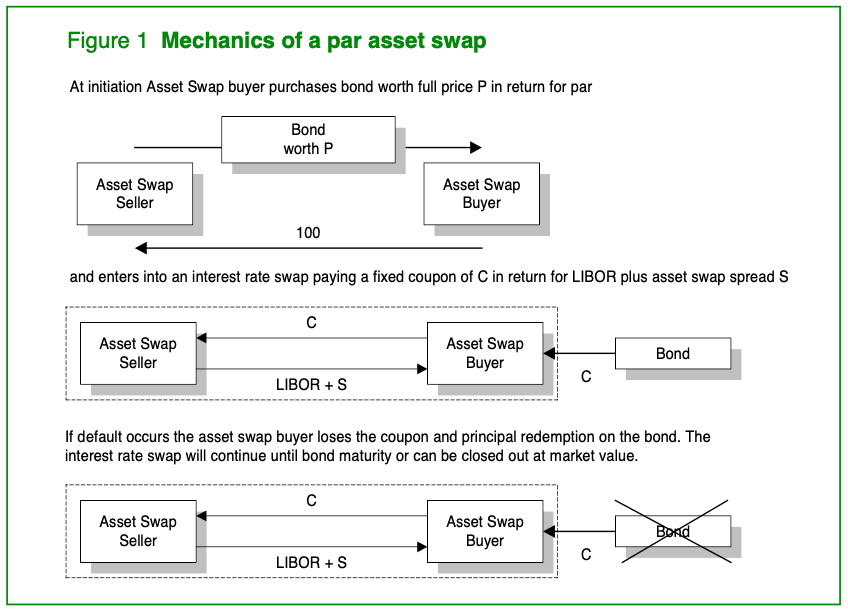
\includegraphics[width=0.7\linewidth]{images/asset_swap}
	\end{center}
\end{frame}

\subsection{Asset Swap Valuation}
\begin{frame}{Valuation of the Asset Swap}
	At valuation time $t$ the \emph{three} following facts are observed:
	\begin{itemize}
		\item<2-> the AS buyer buys a generic \emph{risky} coupon bond at the market price $\overline{\textbf{CBP}}(t,T,K,1)$;
		\item<3-> the AS seller pays/receives to/from the asset swap buyer the difference $\Delta = \overline{\textbf{CBP}}(t,T,K,1)-1$ in such a way that the net sum paid from the AS buyer is always 1; 
		\begin{itemize}
			\item \textcolor{red}{if the bond trades above par} the difference $\Delta$ is paid to the AS buyer by the seller;
			\item conversely \textcolor{red}{if the bond trades below par} the difference $\Delta$ is paid to the AS seller by the buyer.
		\end{itemize}
		\item<4-> A swap is then started between the two counter-parties such that the AS seller receives a fixed leg equal to the coupon stream of the bond and the AS buyer receives the floating leg given by EURIBOR rate plus a \textcolor{red}{spread ($s$)} (again for simplicity the floating payment dates are the same as the fixed leg ones).
	\end{itemize}
\end{frame}

\begin{frame}{Valuation of the Asset Swap}
	\begin{itemize}
		\item From the perspective of the Asset Swap seller the value of the package is given by (we are considering spot trading so $T_\alpha = t = 0$)
		\begin{equation}
			\begin{aligned}
				\textbf{AS}=1&-\overline{\textbf{CBP}}+K\sum_{i=1}^{\beta}\tau_i P(0,T_i)-\sum_{i=1}^{\beta}\tau_i P(0,T_i)(L(T_{i-1},T_i)+s) =\\
				=1&-\overline{\textbf{CBP}}+K\sum_{i=1}^{\beta}\tau_i P(0,T_i)\\
				&-\sum_{i=1}^{\beta}\tau_i P(0,T_i)L(T_{i-1},T_i)-\sum_{i=1}^{\beta}\tau_i P(0,T_i)s=0
			\end{aligned}
			\label{eq:asset_swap_value}
		\end{equation}
	\end{itemize}
\end{frame}

\begin{frame}{Valuation of the Asset Swap}
	\begin{itemize}
		\item We can replace the future rates with the forward rates definition in terms of ZCB, and by its definition (\cref{eq:forward_rate_definition})
		\begin{equation*}
			\begin{aligned}
			\sum_{i=1}^\beta &\tau_i P(0,T_i)F(t;T_{i-1},T_i) =  \sum_{i=1}^\beta \cancel{\tau_i P(0,T_i)}\frac{P(0,T_{i-1})-P(0,T_i)}{\cancel{\tau_i P(0,T_i)}} = \\
			= &P(0,0) \cancel{- P(0,T_1)} + \cancel{P(0,T_1)} \cancel{- P(0,T_2)} + \cancel{P(0,T_2)} + \\
			&\ldots \cancel{- P(0, T_{\beta-1})} \cancel{+ P(0, T_{\beta-1})}-P(0,T_\beta) = 1-P(0,T_\beta) 
			\end{aligned}
		\end{equation*}
		\item Substitute into \cref{eq:asset_swap_value} to get
		\begin{equation*}
			\begin{aligned}
				\textbf{AS}=1&-\overline{\textbf{CBP}}+K\sum_{i=1}^{\beta}\tau_i P(0,T_i) -(1-P(0,T_\beta))
				+ \sum_{i=1}^\beta\tau_i P(0,T_i)s=0
			\end{aligned}
		\end{equation*}
	\end{itemize}
\end{frame}

\begin{frame}{Valuation of the Asset Swap}
	\begin{itemize}
		\item Canceling out the 1s
		\begin{equation*}
			\begin{aligned}
				\textbf{AS}=&-\overline{\textbf{CBP}}+K\sum_{i=1}^\beta\tau_i P(0,T_i) + \\
				& + P(0,T_\beta) + \sum_{i=1}^{\beta}\tau_i P(0,T_i)s=0
			\end{aligned}
		\end{equation*}
		\item Finally we know that
		\begin{equation*}
			\textbf{CBP} = P(0,T_\beta) + K\sum_{i=1}^\beta\tau_i P(0,T_i)
		\end{equation*}
		represents the price of coupons and principal of a  risk-free bond which can be denoted by \textbf{CBP}.
	\end{itemize}
\end{frame}

\subsection{Asset Swap Spread}
\begin{frame}{Asset Swap Spread}
	Solving for $s$ we arrive at the final expression
	\begin{equation}
		\boxed{s = \frac{\textbf{CBP}-\overline{\textbf{CBP}}}{\sum_{i=1}^{\beta}\tau_iP(0,T_i)}}
	\end{equation}
\myendproof
	\begin{itemize}
	\item<2-> An asset swap enables an investor to buy a fixed rate bond and then hedge out the interest rate risk by swapping the fixed payments to floating. In doing so the investor retains the credit risk of the bond but earns a corresponding return. 
	\item<3-> The investor is \emph{still exposed to the loss of the coupons and redemption on the bond}, i.e. the difference between bond and recovery value.
	\item<4-> In economic terms the purpose of the Asset Swap Spread is to compensate the Asset Swap buyer for taking these risks, which is \textbf{measured} by the spread. If the credit worthiness of the issuer reduces ($\overline{\textbf{CBP}}$ decreases), rates remain constant, so $s$ increases.
	\end{itemize}
\end{frame}

\begin{frame}{Asset Swap: Credit Considerations}
	\begin {itemize}
%	\item If the bond defaults, the AS buyer has to continue paying on the swap, which can no longer be funded with the coupon from the bond, or the swap can be closed out at market value. The asset swap buyer also loses the par redemption of the bond, receiving whatever recovery rate the bond issuer pays. 
	\item A trader may want to hedge anyway the credit risk carried on with the asset swap entering into a \emph{Credit Default Swap (CDS)}.
	\item A CDS is a credit insurance contract where the protection buyer pays \emph{spread} ($s_{CDS}$) and in case of a credit event, the protection seller must pay the contingency payment so that the buyer receives no losses from the default.
	\end{itemize}
\begin{center}
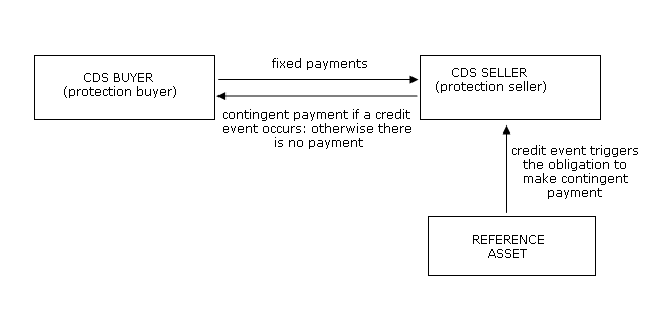
\includegraphics[width=0.7\linewidth]{images/credit-default-swaps}
\end{center}
\end{frame}

\begin{frame}{Asset Swap: Credit Considerations}
	\begin {itemize}
	\item Like $s_{AS}$, also $s_{CDS}$ is quoted on the market, tracking the perceived credit worthiness of the underlying reference entity.
	\item To avoid arbitrage opportunities, $s_{AS}$ of bond with maturity $T$ must be very close to corresponding maturity CDS spread $s_{CDS}$
	\begin{itemize}
		\item if $s_{AS} - s_{CDS} > 0$ the investor can buy the bond, financing the purchase, enters in AS and buying protection, making an (almost) risk free profit (\emph{negative basis trading});
		\item if $s_{AS} - s_{CDS} < 0$ can do the opposite.
	\end{itemize}
	\end{itemize}
\end{frame}

\begin{frame}{Bond and Default}
\begin{itemize}
\item How does the bond price change with non-zero default probability for the issuer ?
\item For simplicity consider a zero coupon bond, with a flat probability of default $p_{\text{def}}$ and a recovery rate $R$.
The price of the bond will be
\begin{equation*}
\begin{cases}
D_f\cdot R \cdot N\quad\text{ with default} \\
D_f\cdot N\quad \text{ with no default}
\end{cases}
\end{equation*}
\begin{columns}
\column{0.5\linewidth}
\item But we know the probability of default so the price estimate will be
\begin{equation*}
\mathbb{E}(\textbf{ZCB}) = p_{\text{def}}\cdot(D_f\cdot R\cdot N) + (1 - p_{\text{def}})(D_f\cdot N)
\end{equation*}
This formula can be easily extended to coupon bearing bonds.
\column{0.4\linewidth}
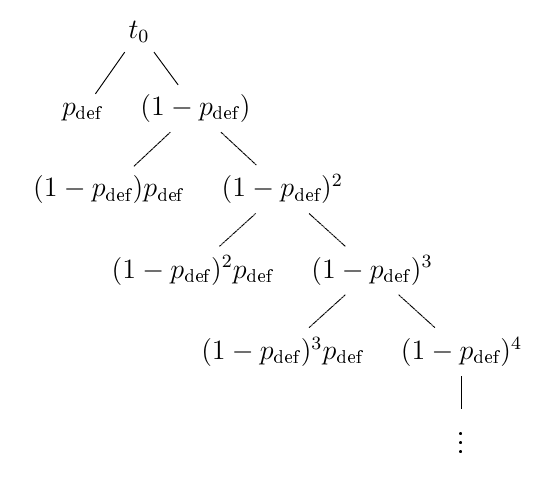
\includegraphics[width=0.9\linewidth]{images/default_tree}
\end{columns}
\end{itemize}
\end{frame}

\begin{frame}[fragile]{ASWP Spread and Default Probability}
Consider ASWP on a 5Y fixed rate bond (yearly coupons 3\%). If the counterparty has nonull default probability, let's see how ASWP spread varies.

\begin{columns}
\column{0.5\linewidth}
\begin{ipython}
import numpy as np

pds = np.arange(0, 1.0, 0.01)

bond = FixedRateBond(today, 0.03, "5y", "1y", 100)
asw = ParAssetSwap(bond)

spreads = []
prices = []
for pd in pds:
  market_price_bond = bond.npv_default(dc, pd=pd, R=0.4)
  prices.append(market_price_bond)
  spreads.append(asw.asspread(dc, pd))    
\end{ipython}
\column{0.5\linewidth}
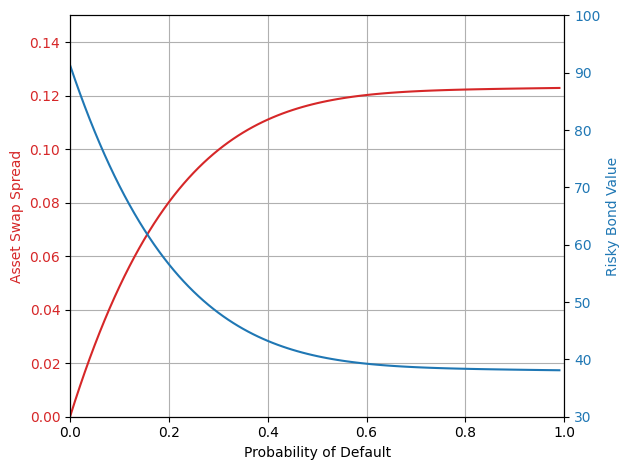
\includegraphics[width=0.9\linewidth]{images/aswp_spread}
\end{columns}

\end{frame}

\begin{homework}
\begin{frame}{\textcolor{white}{Homework}}
\begin{itemize}
\item[white] Describe the asset swap contract for a coupon bond with coupons equal to \textbf{C} and dirty Price equal to $P(t)$. What will happen to the price if the spread increases, all the rest being equal ? What does it mean in term of credit quality expectation by the market for the bond's issuer ?
\item[white]  Consider the 10-year German Bund DBR 0.5\% 2026 which is currently trading at a clean price of 104.58. 
Given that the 10-year EUR swap rate is 0.44\% what is the par-par asset swap spread for this bond ? 
For this exercise assume that all annuity factors have a value of 10.0 for simplicity.
\item[white] Consider the 10-year Greek Government Bond GGB 3.0\% 2026 which is currently trading at a clean price of 75.280. Given that the 10-year EUR swap rate is 0.440\% what is the par-par asset swap spread for this bond ?
\end{itemize}
\end{frame}
\end{homework}

\section{Risk Measures}
\begin{frame}{Sensitivity}
\begin{itemize}
\item The assignment of the correct price to a derivative is not the whole story.
\item \emph{Sensitivity} measures how much the value of a financial instrument changes in response to a change in an underlying factor.  
\item Understanding sensitivity helps investors to:
\begin{itemize}
    \item \emph{Assess Risk:} identify potential vulnerabilities and understand how different market movements can impact portfolio value;
    \item \emph{Manage Portfolios:} make informed decisions about asset allocation and hedging strategies to optimize risk-return profiles;
    \item \emph{Compare Investments:} evaluate the relative risk and potential reward of different investments based on their sensitivities.
\end{itemize}
\item The sensitivity concept closely resamble the mathematical definition of \emph{derivative}, so in the very end estimating the sensitivity is as simple as computing a ratio of variations.
\end{itemize}
\end{frame}

\begin{frame}{Sensitivity}
There are several metrics to estimate the risk and different ways to measure its actual value:
\begin{itemize}
\item \textbf{Duration:} measures a bond's sensitivity to changes in interest rates (higher duration greater price change for a given interest rate shift)
\begin{equation*}
D(y)\equiv -\cfrac{1}{P}\cdot \cfrac{\partial P}{\partial y}=-\cfrac {\partial \ln(P)}{\partial y}\quad\text{ definition as derivative}
\end{equation*}
Its interpreation as sensitivity of a bond's market price to interest rate (i.e. yield) movements comes from
\begin{equation*}
D\approx -\cfrac {1}{P}\cfrac{\Delta P}{\Delta y}\rightarrow \Delta P\approx -P\cdot D\cdot \Delta y
\end{equation*}
Thus duration is approximately equal to the percentage change in price for a given finite change in yield.
\item \textbf{Beta:} measures a stock's sensitivity to changes in the overall market ($\beta > 1$ indicates higher volatility than market).
\item \textbf{Delta:} measures an option's sensitivity to changes in the price of the underlying asset.
\end{itemize}
\end{frame}

\begin{frame}{Sensitivity Calculation}
Sensitivities can be computed with different techniques:
\begin{itemize}
	\item \textbf{analytical}: involves deriving a closed-form expression which can be complex (and not always feasible);
	\item \textbf{numerical}: one bumps the yield curve calibration instruments and reprice the derivative. The change in price gives the risk;
	\item \textbf{curve Jacobians}: when yield curves have been calibrated, the solver slope 'Jacobian' can be kept and used to give the change in derivative price for a change in forwards/discount factors;
	\item \textbf{algorithmic differentiation}: can be used to compute risk "automatically" at the same time as computing the price. It produces accurate and fast risk estimates.
\end{itemize}
\end{frame}

\begin{frame}{Sensitivity in IRD World}
\begin{itemize}
\item<1-> The concept of risk on interest rate derivatives measures precisely the risk associated with the shift of the interest rate curve. 
\item<2-> However there are a number of complications...
\item<2-> Interest rate derivatives depend on a variety of instruments, used in the determination of the interest rate curve, rather than a single asset.
\item<3-> Because there are many ways of shifting the interest rate curve, many different deltas can be computed. 
\end{itemize}
\end{frame}

\begin{frame}{PV01}
\begin{itemize}
    \item<1-> \textcolor{red}{PV01} refers to present value of 1 basis point and it's the discounted value of the cashflows for a rate of 0.01\% for all periods of a particular instrument, (i.e. the NPV of the fixed leg with a rate of 0.01\%).
	\begin{equation}
	   \textbf{PV01} = 0.01\% \frac{\partial \textbf{PFS}}{\partial K} = 0.01\% \sum_{i=\alpha+1}^\beta\tau_iP(t,T_i)
	\end{equation}
	\item<2-> This is a useful measure for dealers calculating the exact P\&L generated by applying a spread (or margin) to a fixed rate away from the mid-market rate.
   \item<3-> Besides giving you the information on how a currency amount would affect the fixed rate (incorporate a fee for example), the PV01 is not useful as a risk measure. 
\end{itemize}
\end{frame}

\begin{frame}{DV01}
\begin{itemize}
	\item<1-> \textcolor{red}{DV01} refers to dollar (actually currency amount) value of 1 basis point and it's the change in value of the NPV of the instrument with a change of 1 basis point in the curve(s). The average of the change for -1bp and +1bp to be more precise. 
	\item<2-> You can consider what happens to the NPV if every rate $r_i$ is changed in parallel by the same amount
	\begin{equation*}
	\textbf{DV01} = \sum_j \frac{\partial \textbf{PFS}}{\partial r_j} = -\sum_{j}\tau_jP_j+\sum_{j}\left(K\sum_{i=\alpha+1}^\beta\tau_i\frac{\partial P_i}{\partial r_j} - \sum_{k=\alpha+1}^\beta L_k\tau_k\frac{\partial P_k}{\partial r_j}\right)
	\end{equation*}
	\item<3-> In the multi-curve framework DV01 would be calculated for the forecast curve, and for the discounting curve, resulting in two actual DV01 measurements.
    \item<4-> When the swap is at fair value (NPV = 0), PV01 and DV01 are very very close although not exactly the same, otherwise they will be different.
    %\item<5-> For given set of market data, changing the swap rate will not change the PV01 but will change the DV01.
    \item<5-> A trader care mostly about DV01 (as a number or, better yet, divided into buckets) because wants to know how the P\&L changes if the curves change by 1bps.
\end{itemize}
\end{frame}

\begin{frame}{DV01 Numerical Calculation}
\begin{itemize}
	\item<1-> Assume the P\&L on a Swap could be approximated with a linear term plus its convexity
	\begin{equation*}
	\Delta \textbf{PFS}(\delta r)\approx \frac{\partial \textbf{PFS} }{\partial r}\delta r + \frac{1}{2}\frac{\partial^2 \textbf{PFS}}{\partial r^2}\delta r^2
	\end{equation*}
	\item<2-> Then bumping $\delta r$ by $\pm 1$~bp and dividing by 2 eliminates the convexity element and very accurately approximates the DV01
	\begin{equation*}
	\textbf{DV01} = \frac{\Delta \textbf{PFS}(+1~bp)-\Delta \textbf{PFS}(-1~bp)}{2}=\frac{\partial \textbf{PFS} }{\partial r}
	\end{equation*}
	\item<3-> Another common method of calculation is to use a single bumped curve by, say, $\frac{1}{100}$th of a bp, and scale the result by 100 (less accurate, since the convexity is marginalised and not eliminated)
	\begin{equation*}
	100\Delta \textbf{PFS}\left(\frac{1}{100}~bp\right)=\frac{\partial \textbf{PFS}}{\partial r}+\frac{1}{200}\frac{\partial^2\textbf{PFS}}{\partial r^2}
	\end{equation*}
	\end{itemize}
\end{frame}

\begin{frame}{Market Rate Sensitivity}
\begin{itemize}
	\item<1-> Forecast and discount curves used in pricing formulas are those \emph{implied} by the market quotes of interest rate instruments (i.e. futures, OIS, etc\ldots). They are usually determined through a technique called \textbf{bootstrap}.
	\item<2-> Another popular, though more complicated, method to assess the risk is to shock each input instrument used in the bootstrapping by 1~bp one by one, rebuild the curves, and then re-price the instrument of interest to obtain its curve sensitivity. 
	\item<3-> This is called \textcolor{red}{Market Rate Sensitivity} and its value is given by the sum of each Swap $NPV$ variations.
	\item<4-> This of course is not quite a "parallel" shift of any curve (e.g. a 1~bp change in futures rate won't correspond to a 1~bp change in the others).
\end{itemize}
\end{frame}

\begin{frame}{Market Rate Sensitivity}
In a plain vanilla Swap is very close but not equal to DV01. The mark to market value of the Swap is \textcolor{red}{not linear} (as in a future contract), but rather it is a \textcolor{red}{convex} function of the rates (just like a bond is a convex function of the yield).
\begin{center}
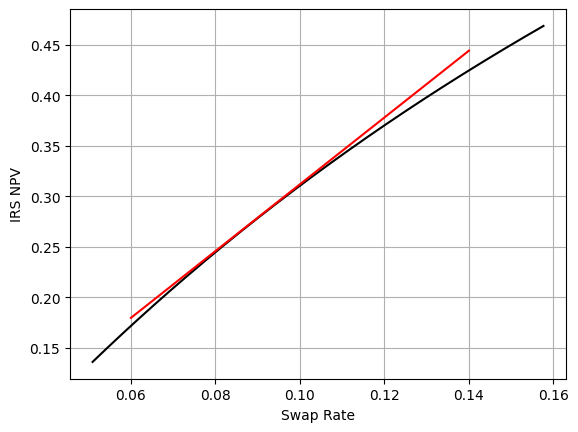
\includegraphics[width=0.5\linewidth]{images/dv01}
\end{center}
\end{frame}

\begin{frame}[fragile]{Algorithmic Differentiation}
Consider the following function
\begin{equation*}
\begin{cases}
\text{Function: } f(x_0, x_1) = 2x_0^2 + 3x_1\\
\text{Solution: } \frac{df}{dx_0} = 4x_0, \text{ and } \frac{df}{dx_1}=3
\end{cases}
\end{equation*}
\begin{columns}
\column{0.4\linewidth}
Let's try to compute its derivative by explicitly defining the $f'$ and using the adjoint technique, when $x_0=2$ and $x_1=3$,

\begin{equation*}
\frac{df}{dx_0} = 8, \text{ and } \frac{df}{dx_1}=3
\end{equation*}
\column{0.6\linewidth}
\begin{ipython}
import numpy as np, tensorflow as tf

def f(x):
  return 2*x[0]**2+3*x[1]

def df_tangent(x):
  return 4*x[0], 3

def df_adjoint(x):
  x = tf.Variable(x, dtype='float', name='x')
  with tf.GradientTape() as tape:
    f = 2*x[0]**2+3*x[1]
  return tape.gradient(f, x)

x = (2, 3)
print (df_tangent(x), df_adjoint(x))
\end{ipython}
\begin{ioutput}

(8, 3) tf.Tensor([8. 3.], shape=(2,), dtype=float32)
\end{ioutput}
\end{columns}
\end{frame}

\begin{frame}[fragile]{Algorithmic Differentiation Example}
Compute DV01 for a 5-years receiver IRS with a 1M notional, exchanging a fixed rate of 5\% with a flat 1\% EURIBOR rate with annual payments.

The explicit derivative is
\begin{equation*}
\begin{gathered}
\cfrac{\partial PV_{float}}{\partial F} = \cfrac{\partial}{\partial F}\sum_i N\tau F_i e^{-rt_i} = \sum_i N\tau e^{-rt_i} \\
\cfrac{\partial PV_{fix}}{\partial r} = \cfrac{\partial}{\partial r}\sum_i N\tau K e^{-rt_i} = -\sum_i N\tau K t_i e^{-rt_i}        
\end{gathered}
\end{equation*}
\end{frame}

\begin{frame}[fragile]{Algorithmic Differentiation Example}
\begin{columns}
\column{0.5\linewidth}
\begin{ipython}
import numpy as np
import tensorflow as tf

class Swap:
  def __init__(self, notional, fixed_rate, tau, terms, rates):
    self.N = notional; self.K = fixed_rate
    self.tau = tau; self.t = terms
    self.r = tf.Variable(rates, name="rates", dtype=tf.float64)

  def swap_price(self, dr=0.0001):
    fixed_pv = tf.Variable(0.0, dtype=tf.float64)
    float_pv = tf.Variable(0.0, dtype=tf.float64)

    with tf.GradientTape(persistent=True) as tape:
      for i in range(1, len(self.t)):
        fixed_pv = fixed_pv + self.K*self.tau
                   *tf.math.exp(-self.r[i]*self.t[i])
      for j in range(1, len(self.terms)):
        F = (self.r[j]*self.t[j]-self.r[j-1]*self.t[j-1])
        float_pv = float_pv + F*tf.math.exp(-self.r[j]*self.t[j])
    
    fixed_pv_dot = np.sum(dr*tape.gradient(fixed_pv, self.r))
    float_pv_dot = np.sum(dr*tape.gradient(float_pv, self.r))

    swap_pv = self.N*(fixed_pv - float_pv)
    swap_pv_dot = self.N*(fixed_pv_dot - float_pv_dot)

    return swap_pv, swap_pv_dot
\end{ipython}
\column{0.5\linewidth}
\begin{ipython}
N = 1e6
fixed_rate  = 0.015
tau         = 1.0
terms       = np.array([0.0, 1.0, 2.0, 3.0, 4.0, 5.0])
rates       = np.array([0.01, 0.012, 0.013, 0.014, 0.016, 0.017])

swap = Swap(N, fixed_rate, tau, terms, rates)
price, dv01 = swap.swap_price()

print (f"Swap price: {price:,.2f}")
print (f"DV01: {dv01:,.2f}")
\end{ipython}
\begin{ioutput}

Swap price: -9,097.43
DV01: -472.60
\end{ioutput}
\end{columns}
\end{frame}

%https://quant.stackexchange.com/questions/49582/interest-rate-swap-pv01-vs-dv01
%https://quant.stackexchange.com/questions/70346/fixed-vs-float-swap-interest-rate-risk/70426#70426
%https://math.nyu.edu/~avellane/DerivativeSecurities7.pdf

%1) Why does an interest rate swap have no duration, but it does have a DV01?

%Every spread product has duration and DV01 since all are sensitive to underlying moves in rates. To calc duration on a swap it's your notional/DV01 * 10k. As your swap reaches maturity the duration and DV01 factors down. Longer duration swaps, say 10Y vs 2Y, will inherently have more duration. Ex. a 10Y swap will have a duration slightly less than 10 depending on how much time to maturity left on the position.  
%
%For 2 and 3, do not think of each leg of the swap having DV01. Rather, the entire swap itself (both legs) is one position with DV01 depending on if you are paying/receiving fixed vs float.
%
%2) What does it mean for the fixed leg of an interest rate swap to have positive DV01?
%
%If you pay fixed and receive float, the entire swap has a positive DV01. Rates sell off (go higher), and you receive positive PnL on the position = positive DV01.


%%\begin{frame}{Trading and Hedging Swaps}
%%	For example, the yield spread is 0.6524\%. An investor believes that this yield spread will narrow as inter-bank credit improves relative to German Sovereign credit. By entering into a position which profits from a rise in the lower (German	Sovereign) yields and / or a fall in the higher (inter-bank) yields, the investor is able to express his view on relative credit pricing.
%%	AGGIUNGERE UN PO' DI SPIEGAZIONE
%%\end{frame}

\begin{homework}
\begin{frame}{\textcolor{white}{Homework}}
\begin{itemize}
\item[white] Consider a 2-year Interest Rate Swap on a notional of 1M, with a fixed rate of 5\% and paying Libor rate annually. The term-structure of interest rates is flat at 5\%.
Estimate the DV01 of the swap numerically.  
\end{itemize}
\end{frame}
\end{homework}

\section{Cap and Floor}
\begin{frame}{Caps and Floors}
	\begin{itemize}
		\item<1-> A \textcolor{red}{Cap} is a Payer IRS in which the payment is done only if the payoff is positive. Its value is the expectation of 
		\begin{equation}
			\sum_{i=\alpha+1}^{\beta}D(t,T_i)N\tau_i\max\left[L(T_{i-1},T_i)-K,0\right]
			\label{eq:cap}
		\end{equation} 
		\item<2-> The cap allows investors which have a debt at a variable rate to buy insurance against high rates in the future.
		\item<3-> A \textcolor{red}{Floor} is the same kind of object but analogous to a Receiver IRS:
		\begin{equation}
			\sum_{i=\alpha+1}^{\beta}D(t,T_i)N\tau_i\max\left[K-L(T_{i-1},T_i),0\right]
			\label{eq:floor}
		\end{equation} 
	\end{itemize}
\end{frame}

\subsection{Caplets}
\begin{frame}{Caplet and Floorlet}
	\begin{itemize}
		\item<1-> Considering each element of the sum in \cref{eq:cap} or \cref{eq:floor} we see that Cap/Floor can be split into forward starting options over a floating rate, called \textcolor{red}{Caplet/Floorlet}.
		\item<2-> A Caplet/Floorlet payoff is defined as
		\begin{equation*}
			D(t,T_i)N\tau_i\max\left[L(T_{i-1},T_i)-K,0\right]
		\end{equation*} 
		and its value is given by
		\begin{equation}
			\textbf{Cpl}(t,T_{i-1},T_i,\tau,N,K)=\expect{Q}\left[e^{-\int_t^{T_i}r_s ds}N\tau(L(T_{i-1},T_i)-K)^+ | \mathcal{F}_t\right]
		\end{equation}
		\item<3-> This can also be written
		\begin{equation*}
			\textbf{Cpl}=N\expect{Q}\left[e^{-\int_t^{T_{i-1}}r_s ds}\tau P(T_{i-1},T_i)(L(T_{i-1},T_i)-K)^+ | \mathcal{F}_t\right]
		\end{equation*}
	\end{itemize}
\end{frame}

\begin{frame}{Caplets as ZCB Options}
	\begin{itemize}
		\item<1-> Using the LIBOR rate definition we get
		\begin{equation*}
			\begin{aligned}
				\textbf{Cpl} &=N\expect{Q}\left[e^{-\int_t^{T_{i-1}}r_s ds}P(T_{i-1},T_i)\left(\frac{1}{P(T_{i-1},T_i)}-1-K\tau\right)^+ \Big\rvert \mathcal{F}_t\right] \\
				& = N\expect{Q}\left[e^{-\int_t^{T_{i-1}}r_s ds}\left(1-(1+K\tau)P(T_{i-1},T_i)\right)^+ | \mathcal{F}_t\right]
			\end{aligned}
		\end{equation*}
		\item<2-> Multiplying by $\frac{1}{1+K\tau}$ we finally get
		\begin{equation}
			\boxed{\textbf{Cpl}=N(1+K\tau)\expect{Q}\left[e^{-\int_t^{T_{i-1}}r_s ds}\left(\frac{1}{1+K\tau}-P(T_{i-1},T_i)\right)^+ \Big\rvert \mathcal{F}_t\right]}
		\end{equation}
	\end{itemize}
\end{frame}

\begin{frame}{Caplets as ZCB Options}
	\begin{block}{Intepretation}
		\begin{enumerate}
		\item Caplets can be seen as \textcolor{red}{put options} on ZCBs
\begin{equation*}
\textbf{Cpl}=N'\expect{Q}\left[D(t,T_{i-1})\left(K'-P(T_{i-1},T_i)\right)^+ \Big\rvert \mathcal{F}_t\right]
\end{equation*}
		\item Similarly floorlets are \textcolor{red}{call options} on ZCBs
\begin{equation}
\textbf{Flr}=N'\expect{Q}\left[D(t, T_{i-1})\left(P(T_{i-1},T_i)-K'\right)^+ \Big\rvert \mathcal{F}_t\right]
\end{equation}
		\end{enumerate}
	\end{block}
\end{frame}

\section{The Black Model}
\begin{frame}{The Black Model - Overview}
	\begin{itemize}
		\item The \textcolor{red}{Black Model} extends the Black-Scholes formula to \emph{caplets} and \emph{swaptions}. % and \emph{bond options}. %It uses the forward coordinates, not the spot ones; this last is not a minor issue indeed.
		\item The main difference with respect to the Black-Scholes set up is that \textcolor{red}{forward rates $F(t;T_{i-1},T_i)$ (or swap rates $S_{\alpha\beta}(t)$) are log-normally distributed}, rather than the spot price of the underlying. 
		\item It should be stated that Black’s formulas did not originally correspond to prices that arise from the application of martingale pricing theory to some particular model. 
		\item The advent of the \emph{market models} will provide a belated justification for these formulas but we shall see that the justifications are mutually inconsistent. 
		\item Indeed, it may be shown that if forward rates have deterministic volatilities then it is not possible for swap rates to also have deterministic volatilities. Therefore Black’s formulas for caplets and swaptions cannot both hold within the same model. 
	\end{itemize}
\end{frame}

%\begin{frame}{The Black Model: Overview}
%	\begin{itemize}
	%		\item It should be recognized that the Black model is being actually used in different ways. In particular the caps uses the forward short-term LIBOR rate as the underlying state variable, whereas the swaptions uses longer-term forward swap rates. Beause forward swap rates are nearly linera in individual forward rates , the lognormality assumption implicit in the Black model cannot hold simultaneously for both, since a linear combination of lognormal variables is not lognormal.
	%	\end{itemize}
%\end{frame}

%\begin{frame}{The Black Model: Overview}
%	\begin{itemize}
%	\item It should be stated that Black’s formulae for caps and swaptions did not originally correspond to prices that arisefrom the application of martingale pricing theory to some particular model. 
%	\item It is widely used in practice as the metric by which traders translated volatilities into prices until rates became too low and the model collapsed under the assumption of positive rates.
%		\item 
%		\item ...but for the moment we cannot consider it as a model ! Just a bunch of formulas.
%		
%
%
%When we model swap rates directly as in (30) we say that we have a swap market model. Thiscontrasts with the LIBOR market models of Section 4.Remark 5 The advantage of Black’s swaption formula is that it is elegant and exact, whereas the BGM formula is cumbersome and only an approximation. However, the BGM approximation is consistent with Black’s formulae for caplets and caps whereas Black’s swaption formula is not. 
%That said, within the LIBOR market framework with deterministic volatilities, it can be argued thatforward swap rates are approximately log-normally distributed.
%
%
%	\end{itemize}
%\end{frame}

\begin{frame}{Pricing Caps with the Black-76 Formula}
	\begin{block}{Definition}
	\begin{equation}
		\begin{aligned}
		\textbf{Cap}_{Bl}(0, \tau,N,K,\sigma_{\alpha,\beta}) &= N\sum_{i=\alpha+1}^{\beta}\textbf{Cpl}_{Bl}(T_i, \tau,K,\sigma_{\alpha,\beta}) = \\ &=N\sum_{i=\alpha+1}^{\beta}\tau P(0,T_i) \textbf{Bl}(K,F(0;T_{i-1},T_i),v_i)
		\end{aligned}
		\label{eq:cap_black}
	\end{equation}
	where
	\begin{equation*}
		\begin{gathered}
			\boxed{\textbf{Bl}(K,F_i,v_i)=F\Phi(d_1(K,F_i,v_i)) - K\Phi(d_2(K,F_i,v_i))} \\
			d_{1,2} = \frac{\log{\cfrac{F_i}{K}} \pm \cfrac{v_i^2}{2}}{2} \\[0.2cm]
			v_i = \sigma_{\alpha,\beta}\sqrt{T_{i-1}}
		\end{gathered}
	\end{equation*}
	\end{block}
\end{frame}

\begin{frame}{Problems with the Black Model}
\begin{itemize}
	\item It is widely used in practice as the metric by which traders translated volatilities into prices until rates became too low and the model collapsed under the assumption of positive rates.
	\item In the Black model \textcolor{red}{negative rates are not allowed}.
	\begin{equation*}
		d_{1,2} = \frac{\boxed{\log{\frac{F}{K}}} \pm \cfrac{v^2}{2}}{2} 
	\end{equation*}
	but in the last years in the inter-bank market it was not so unusual to find prices for -1\% strike floors.
	\item Moreover in the Black model the empirical evidence of the "smile" (volatility vs $K$) is not accounted for, i.e. $\sigma$ is a constant. Two caps identical but for the strike need a different volatility to recover two different market prices if one uses Black formula.
	%\item And this is clear if one looks at the distribution and at the process of $F(t, T, S)$; the volatility does not depend on the strike of the option. It is a characteristic of the forward rate.
\end{itemize}
\end{frame}

\begin{frame}{The Practitioner Solutions}
\begin{itemize}
	\item \textbf{"Smile" issue}: the model is used with \textcolor{red}{different input volatilities for different strikes}. In practice it is a mapping of implied volatilities into prices and vice versa.
	\item \textbf{Non-positive rates}: could have switched to a different dynamics, like ABM, where negative values are "normal". But there are large differences in the tails between normal and log-normal distributions.
	So Black model has been \textcolor{red}{shifted}. The technique was already known but in the last years has become crucial to shift the lower bound of prices admitted by the model.
\end{itemize}
\end{frame}

\begin{frame}{Shifted Log-normal Model for Caplets}
\begin{itemize}
	\item It can be shown that Black formula provides valid solutions if strike and forward rate are \textcolor{red}{shifted}. For a $(T,S)$ caplet with strike $K$ we get
	\begin{equation}
		\textbf{Cpl}_{Bl}(t,T,S,\tau,K,v_T,\alpha) = P(t,S) Bl(K+\alpha,F(t;T,S)+\alpha,v_T)
	\end{equation}
	where $d_1$ and $d_2$ read as before and instead $v_i$ is now given by
	\begin{equation*}
		v_i = \sigma^{\text{shifted}}\sqrt{T_{i-1}}
	\end{equation*}
	\item The market quotes of $\sigma^{\text{shifted}}$ refer to shifts $\alpha$ of the order of [2\%,3\%].
	%\item What is the relationship between $\sigma^{\text{shifted}}$ and $v_T$ ?
	%\item Rewrite the Black-76 SDE for the $(T, S)$ caplet as follows
	%\begin{equation}
	%	dF(t,T,S)=\sigma^{\text{shifted}}(F(t,T,S)-\alpha)dW^{\mathcal{Q}_S}(t)
	%\end{equation}
	%\item It is easy to see that the price for a $(T,S)$ caplet with strike $K$ is given by
	%\begin{equation}
	%	Cpl(t,T,S,\tau,K,v_T,\alpha)=P(t,S)Bl(K-\alpha,F(t,T,S)-\alpha,v_T)
	%\end{equation}
\end{itemize}
\end{frame}

\begin{frame}[fragile]{Shifted Brownian Motion}
\begin{columns}
    \column{0.55\linewidth}
    \begin{ipython}
import numpy as np

def GBM(mu, sigma, X0, T, steps, N):
    X = np.zeros(shape=(steps, N))
    dt = T/steps
    X[0, :] = X0
    eps = np.random.normal(size=(steps-1, N))
    X[1:, :] = np.exp((mu-0.5*sigma**2)*dt+sigma*np.sqrt(dt)*eps)
    return np.cumprod(X, axis=0)

def GBMShifted(mu, sigma, shift, X0, T, steps, N):
    X0_shifted = X0 + shift
    if (X0_shifted < 0.0):
        raise ValueError('Shift is too small !')

    X_shifted = GBM(mu, sigma, X0_shifted, T, steps, N)
    return X_shifted - shift
    \end{ipython}
\column{0.4\linewidth}
\begin{ipython}
N = 10000
tsteps = 500
T = 3.0
sigma = 0.2
L0 = -0.05
shift = 0.1

paths = GBMShifted(0.0, sigma, shift, L0, T, tsteps, N)    
\end{ipython}
\begin{center}
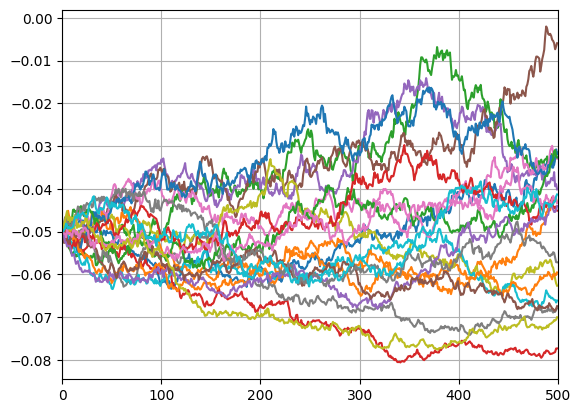
\includegraphics[width=0.9\linewidth]{images/shifted_gbm}
\end{center}
\end{columns}
\end{frame}

\begin{frame}{Shifted Log-normal}
\begin{itemize}
\item The density for the log-normal is:
\begin{equation}
\cfrac{1}{(x-\delta)\sigma\sqrt{2\pi}}e^{-\frac{1}{2\sigma^2}(\ln(x-\delta)-\mu)^2},\quad x>\delta, \mu\in\mathbb{R},\sigma >0
\end{equation}
\item In a \emph{Normal} distribution, $\mu$ plays the role of location-parameter, so "shifting" it is a trivial task.
\begin{columns}
\column{0.6\linewidth}
\item In the log-normal instead $\mu$ is not a shift parameter, but a \emph{scale} parameter. It stretches and compresses rather than shifts ($\sigma$ is a shape parameter, controlling how skewed/heavy tailed the distribution is).
\item Shifting the normal and then exponentiating to a log-normal is different from shifting the log-normal (the issue boils down to the fact that addition and exponentiation are not commutative).
\column{0.4\linewidth}
\begin{center}
    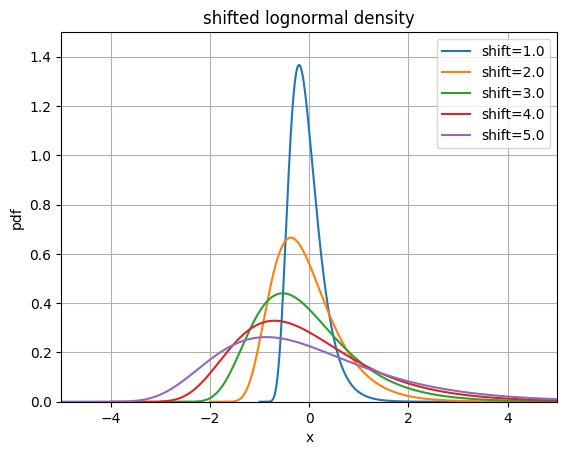
\includegraphics[width=0.95\linewidth]{images/shifted_lognormal}
\end{center}
\end{columns}
\end{itemize}
\end{frame}

\begin{frame}[fragile]{Shifted Black Formula}
Compare the result for Cap Black formula to the Monte Carlo simulation both with a shift $\Delta$.
\begin{columns}
\column{0.5\linewidth}
\begin{ipython}
import numpy as np

def BS_shifted(St, K, shift, r, sigma, ttm):
    K_shifted = K + shift
    St_shifted = St + shift
    return BS(St_shifted, K_shifted, r, sigma, ttm)

T = 3.0
sigma = 0.2
L0 = -0.05
shift = 0.1
r = 0

K = np.linspace(-shift, np.abs(L0)*3, 25)
optPriceMCV = np.zeros([len(K), 1])
for idx in range(len(K)):
  optPriceMCV[idx] = np.mean(np.maximum(paths[-1, :] - K[idx], 0.0))

optPriceExact = BS_shifted(L0, K, shift, r, sigma, T)
\end{ipython}
\column{0.5\linewidth}
\begin{center}
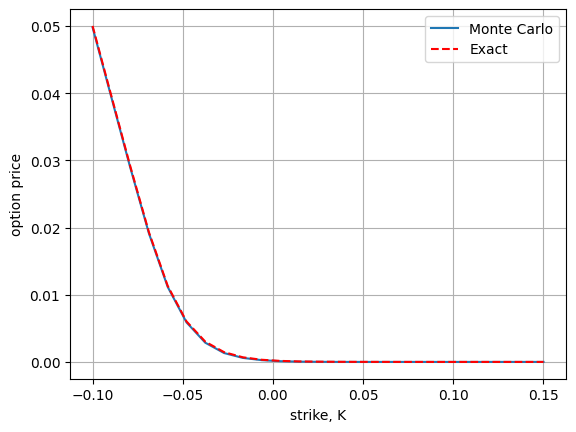
\includegraphics[width=0.65\linewidth]{images/shifted_call_BS_vs_MC}\\
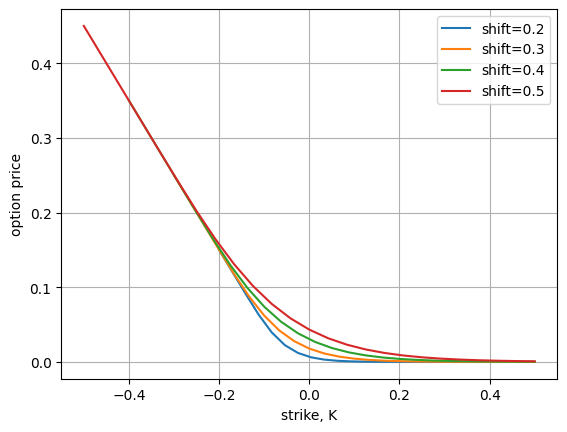
\includegraphics[width=0.65\linewidth]{images/shifted_call}
\end{center}
\end{columns}
\end{frame}


%\begin{frame}{The Volatility Hump}
%\begin{itemize}
%	\item Empirical studies have pointed out two very important facts:
%	\begin{itemize}
%		\item the first one is that interest rates volatility can depend on the level of the interest rates themselves;
%		\item moreover the volatility function is increasing in the short end of the curve, and decreasing in the long end, with an \textcolor{red}{humped} type movement.
%	\end{itemize}  
%	\begin{columns}
%		\column{0.45\linewidth}
%		\item Uncertainty is bigger in the intermediate region and lower in the front of the maturity spectrum. For long maturities volatility tends to decay.
%		\item When the hump does not appear it is regarded as \emph{stressed market}.
%		%\item There is a financial explanation for this feature.
%		\column{0.45\linewidth}
%		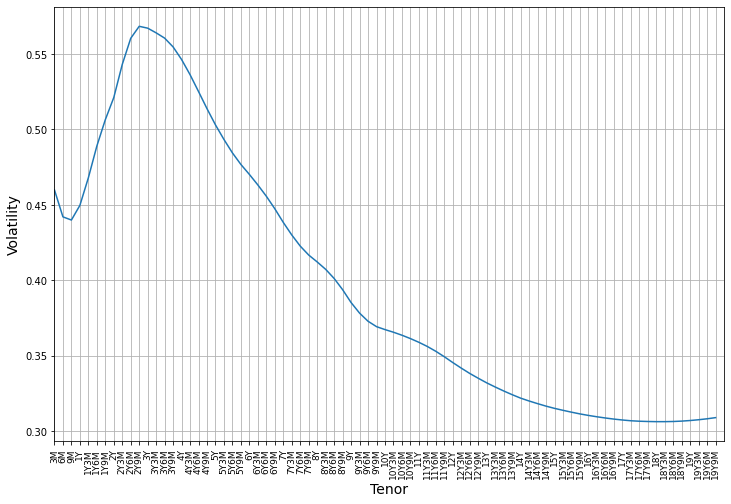
\includegraphics[width=1.1\linewidth]{cap_vola}
%	\end{columns}
%\end{itemize}
%\end{frame}
\end{document}


